%%%%%%%%%%%%%%%%%%%%%%%%%%%%%%%%%%%%%%%%%%%%%%%%%%%%%%%%%%%%%%%%%
\chapter{RESULTS}
\label{ch:CH6}
%%%%%%%%%%%%%%%%%%%%%%%%%%%%%%%%%%%%%%%%%%%%%%%%%%%%%%%%%%%%%%%%%

\section{Performance Measurement}

\subsection{Confusion Matrix}

The confusion matrix is a table that constructed to visualize the performance of a classifier. It includes actual and predicted results for each class on the corresponding task. In our study, the rows specifies the predicted results whereas columns specifies actual ones.

During the performance measurement, the focused class is called as Positive (P), and the others are as Negatives (N). For binary classification problems, which is as in our study, one class can be directly specified as P and the other as N. We indicated the COVID-19 label as Positive class, and the non-COVID-19 label as Negative class. 

If a sample in actual P class is predicted as in P class, then it is a True Positive (TP) sample, otherwise it is False Positive (FP). On the other hand, if a sample in actual N class is predicted as in P class, then it is a False Negative (FN) sample, otherwise it is True Negative (TN). This notations can be seen on Table~\ref{tab:sample_confusion_matrix}.

From the definitions, the following equalities can be easily derived: P = TP + FN and N = FP + TN.

\begin{table*}[!h]
{
    \setlength{\tabcolsep}{14pt}
    \caption{Confusion matrix.}
    \begin{center}
    % \vspace{-6mm}
    \begin{tabular}{|c|c|c|c|}
    \hline
    \multicolumn{2}{|c|}{\multirow{2}{*}{\begin{tabular}[c]{@{}c@{}}\\\\ \end{tabular}}} & \multicolumn{2}{c|}{\textbf{Actual}} \\ 
    \cline{3-4} 
    \multicolumn{2}{|c|}{}                                                                            & \begin{tabular}[c]{@{}l@{}}\quad\quad P \\ (COVID-19)\end{tabular} & \begin{tabular}[c]{@{}l@{}}\quad\quad N \\ (non-COVID-19)\end{tabular} \\ 
    \hline
    \multirow{2}{*}{\textbf{Predicted}}      & \begin{tabular}[c]{@{}l@{}} \quad\quad P \\ (COVID-19)\end{tabular}         & \textbf{TP}                                             & FN                                                          \\
    \cline{2-4} 
                                    & \begin{tabular}[c]{@{}l@{}} \quad\quad N \\ (non-COVID-19)\end{tabular}     & FP                                                      & \textbf{TN}                                                 \\ \hline
    \end{tabular}
    % \vspace{-6mm}
    \end{center}
    \label{tab:sample_confusion_matrix}
}
\end{table*}

Various meaningful ratios can be extracted from the confusion matrix given in Table~\ref{tab:sample_confusion_matrix}. In this section, we study the significant ones which were also used in the thesis to measure the performance of our tasks.

\subsubsection*{Sensitivity}

Sensitivity, or in other words, true positive rate (TPR), measures the ratio of positive class samples predicted correctly over all samples predicted as positive as given below:

\begin{equation}
\label{eq:TPR}
    TPR = \frac{TP}{P} = \frac{TP}{TP + FN}\raisepunct{.}
\end{equation}

\subsubsection*{Specificity}

Specificity, or in other words, true negative rate (TNR),  measures the ratio of negative class samples predicted correctly over all samples predicted as negative as given below:

\begin{equation}
\label{eq:TNR}
    TNR = \frac{TN}{N} = \frac{TN}{FP + TN}\raisepunct{.}
\end{equation}

\subsubsection*{Precision}

Precision, or in other words, positive predictive value (PPV), measures the ratio of correctly predicted positive class samples over all samples having actual positive label as given below:

\begin{equation}
\label{eq:PPV}
    PPV = \frac{TP}{TP + FP}\raisepunct{.}
\end{equation}

\subsubsection*{Accuracy}

Accuracy (ACC) measures the ratio of correctly predicted samples over all samples as given below:

\begin{equation}
\label{eq:ACC}
    ACC = \frac{TP + TN}{P + N} = \frac{TP + TN}{TP + FP + FN + TN}\raisepunct{.}
\end{equation}

\subsubsection*{F1 Score}

F1 Score is the harmonic mean of sensitivity and precision as given below:

\begin{equation}
\label{eq:F1_Score}
    F_{1} = 2 \times \frac{PPV \times TPR}{PPV + TPR} = \frac{2 \times TP}{(2 \times TP) + FP + FN}\raisepunct{.}
\end{equation}

 
\subsubsection*{Area Under the Curve}

Area under the curve (AUC) score measures the probability of classifier to rank a randomly chosen positive sample higher than a random chosen negative sample (under the assumption that "positive" ranks are higher than "negative" ranks) for normalized samples. The computation of AUC score value is as given below:

\begin{align}
\label{eq:AUC_Score}
    \nonumber
    & TPR(t) : t \rightarrow y \left ( x \right ), \\
    \nonumber
    & FPR(t) : t \rightarrow x, \:\: \text{and} \\ 
    & AUC = \int_{0}^{1} TPR \left ( FPR^{-1}\left ( x \right ) \right ) dx = \int_{-\infty}^{\infty} TPR \left ( t \right ) \times {FPR}' \left ( t \right ) dt.
\end{align}


\subsection{Analysis of Confusion Matrix}

We computed each sensitivity, specificity, precision, accuracy, and F1-score metric in a weighted way to achieve and report the metrics for the corresponding model, not for each class separately. In other words, each metric was computed for each class and then the weighted average was taken as given below:

\be
\label{eq:weighted_avg_metric}
\frac{\sum_{i=1}^{m} (\text{the metric value for class i}) \times (\text{the number of test samples in class i})} {(\text{the total number of test samples})} \:\: \raisepunct{.}
\ee

Recall that the task we worked on is a binary classification problem. That is, $m$ was 2 in our computations. So that, the average value for metric $M$ of an experiment, where M is one of Sensitivity, Specificity, Precision, Accuracy and F1-Score metrics, was computed as:

\be
\label{eq:weighted_avg_binary_class_metric}
M = \frac{M_{c_{1}} \times n_{c_{1}} + M_{c_{2}} \times n_{c_{2}}} {n_{c_{1}} + n_{c_{2}}} \:\: \raisepunct{,}
\ee

where $M_{c_{1}},\:\:M_{c_{2}},\:\:n_{c_{1}}\:\:\text{and}\:\:n_{c_{2}}$ refer the value of $M$ for class 1, the value of $M$ for class 2, the number of test samples in class 1 and the number of test samples in class 2, respectively.

\section{Convolutional Neural Network Results}

Here, we report the results of Convolutional neural network experiments explained in Section~\ref{sec:CH5_cnn_experiments}. As stated, AlexNet, ResNet-18, ResNet-34, ResNet-50, VGG-16, and VGG-19 architectures were trained by initialized with their pre-trained weights, and three different optimizers such that SGD with momentum, Adam, and AdamW were used to optimize the cross-entropy loss function. The accuracy and loss curves for three different optimizers on train and validation processes can be viewed on Figures~\ref{fig:alexnet_plots}-\ref{fig:vgg19_plots} where the horizontal axis represents the number of epochs. The plots were created by TensorBoard platform prepared with the Python TensorFlow package version 2.3.1. Additional required package versions are as follows: 1) TensorFlow Addons with the version of 0.11.2, 2) TensorFlow Estimator with the version of 2.3.0, 3) TensorFlow Hub with the version of 0.10.0, and 4) TensorFlow Probability with the version of 0.10.0.

The results can be also seen in Table~\ref{tab:cnn_result_table} including accuracy, sensitivity, specificity, precision and F1 score values, and loss values for last train epoch and test run. We obtained the best result from ResNet-50 model after $9^{th}$ train epoch in 7 minutes with the accuracy, sensitivity, specificity, precision, F1 score and AUC score of 92.16\%, 0.9216, 0.9215, 0.9216, 0.9216, 0.9215 respectively, and the loss of $9^{th}$ train epoch and validation as 0.0223 and 1.3687. \textcolor{purple}{On the other hand, VGG19 is the model that achieves its best at third epoch with Adam optimizer. Moreover, AlexNet model stands out with its stable metric values, which are always around 0.90, for all experimented optimizers. At the angle of last train loss and test loss, VGG16 with AdamW optimizer has the minimum last train loss as 0.0057 and the minimum test loss as 0.0831. ResNet-18 and ResNet-34 models achieved metric values around 0.90; however, they could not reach to ResNet-50 model whose architecture is more deeper than them. Lastly, it is clear that there can be no generalization about optimizers such that one optimizer is always better than other or vice versa.}
 
 % adam, adamw ve sgd momentumda decay ve momentum değerleri tune edilen değerler olduğu için hep farklı değerler alıyor. bazı adam sonuçlarında decay değeri 0 olabiliyor.

\begin{figure}[!h]
    \centering
    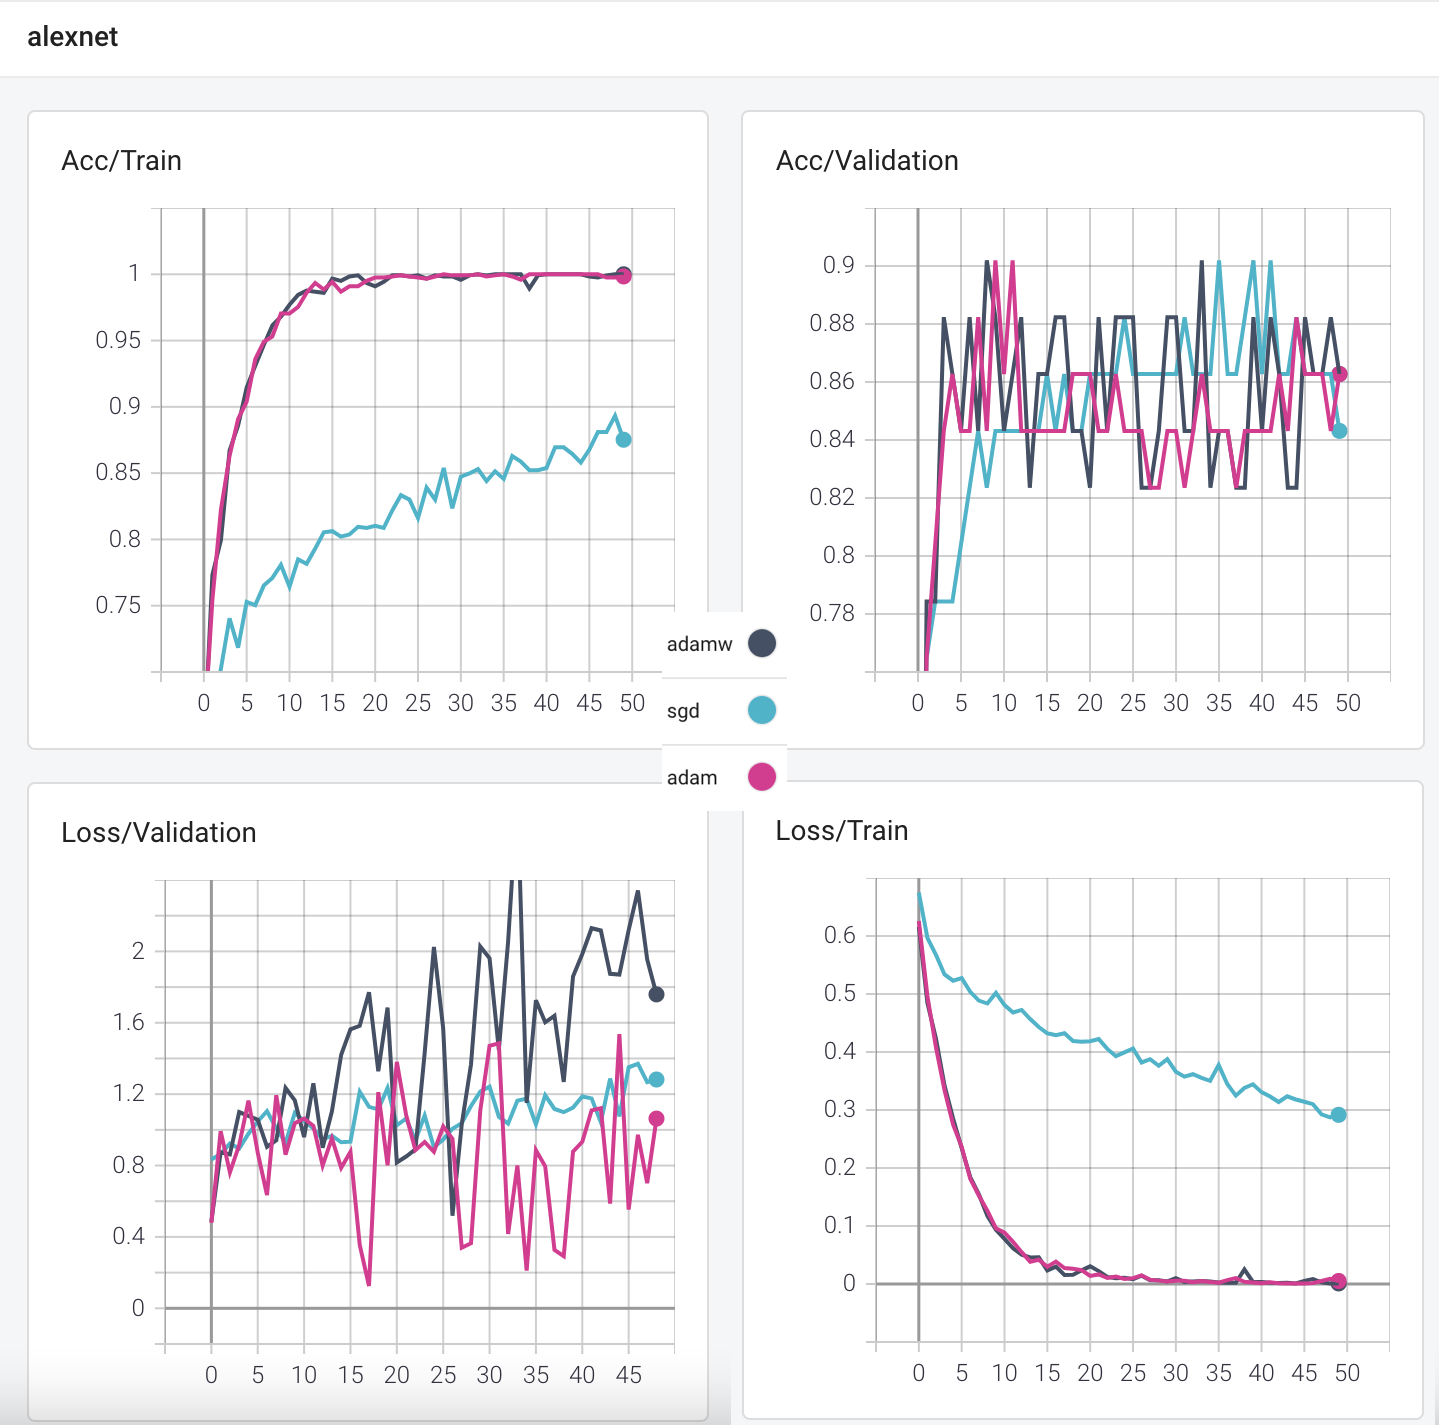
\includegraphics[width=\linewidth]{fig/alexnet.png}
    \vspace{2mm}
    \caption{AlexNet model accuracy and loss curves on train and validation processes with the SGD momentum, Adam, and AdamW optimizers.}
    \label{fig:alexnet_plots}
\end{figure}

\begin{figure}[!h]
    \centering
    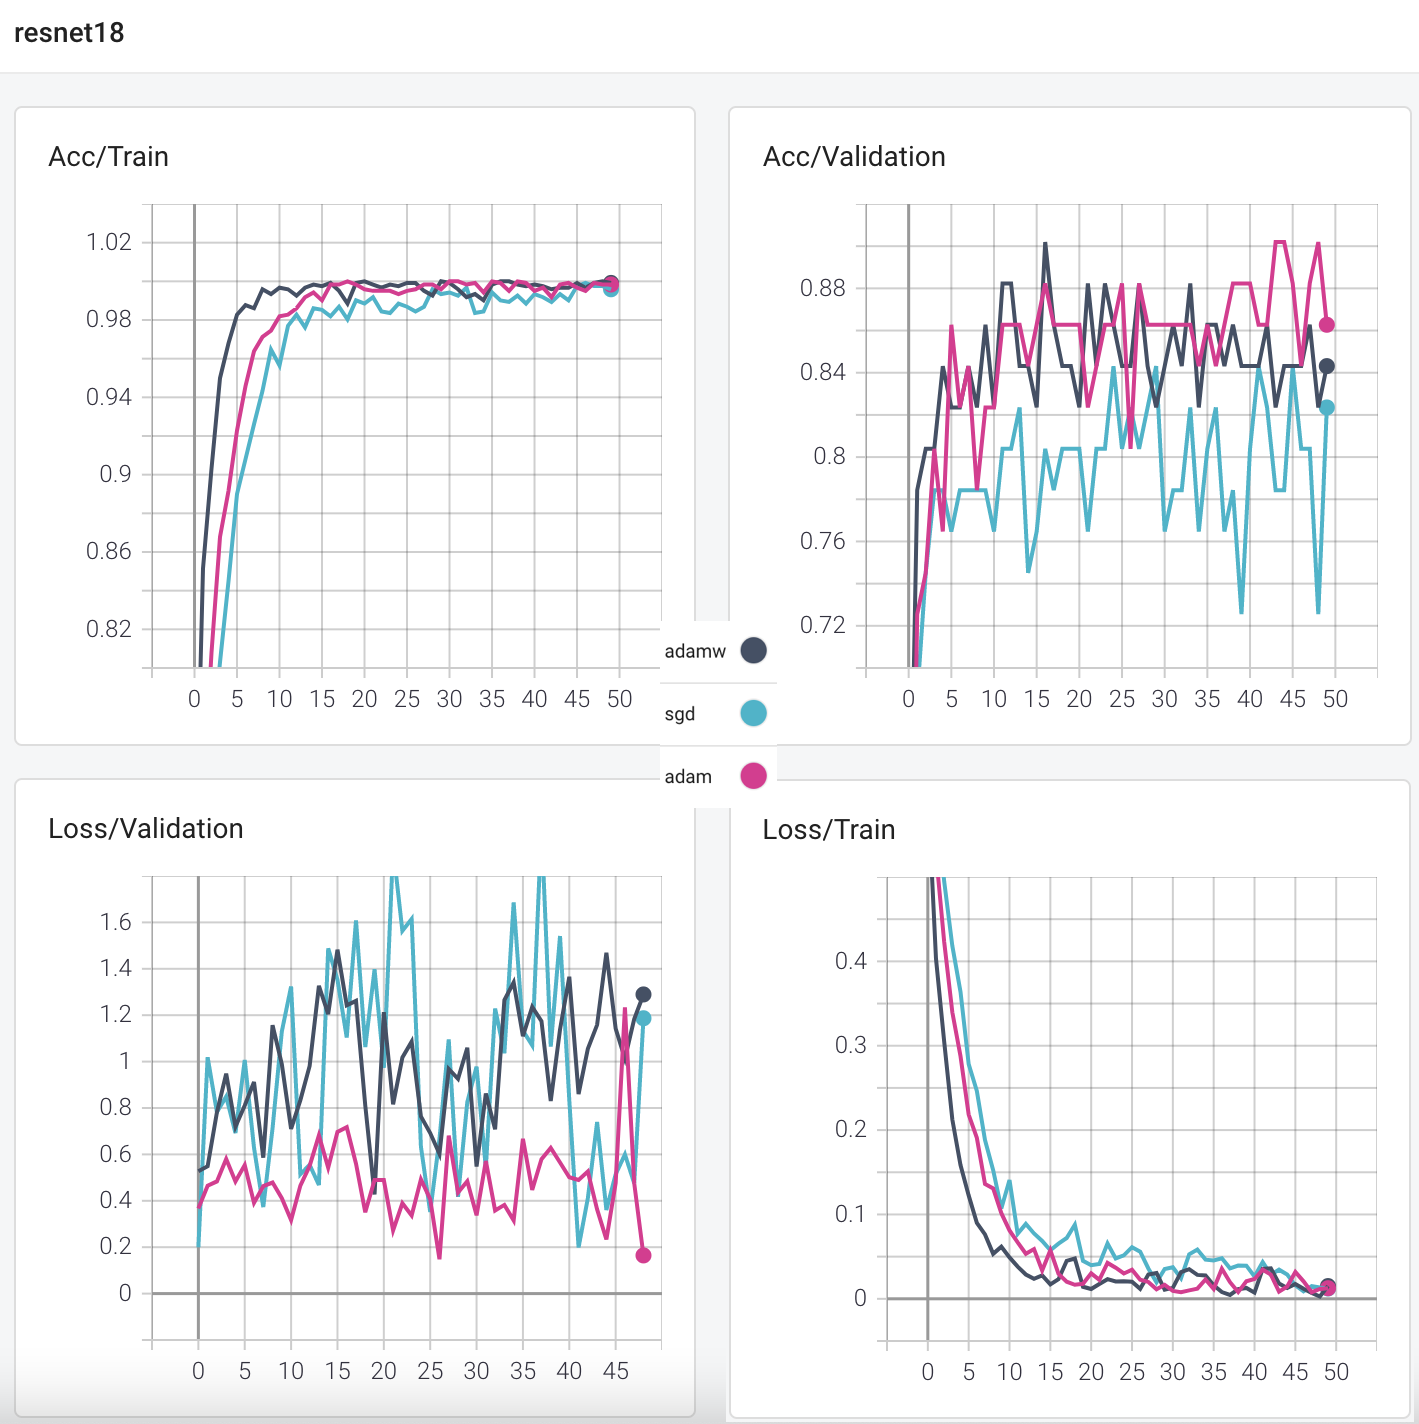
\includegraphics[width=\linewidth]{fig/resnet18.png}
    \vspace{2mm}
    \caption{ResNet-18 model accuracy and loss curves on train and validation processes with the SGD momentum, Adam, and AdamW optimizers.}
    \label{fig:resnet18_plots}
\end{figure}

\begin{figure}[!h]
    \centering
    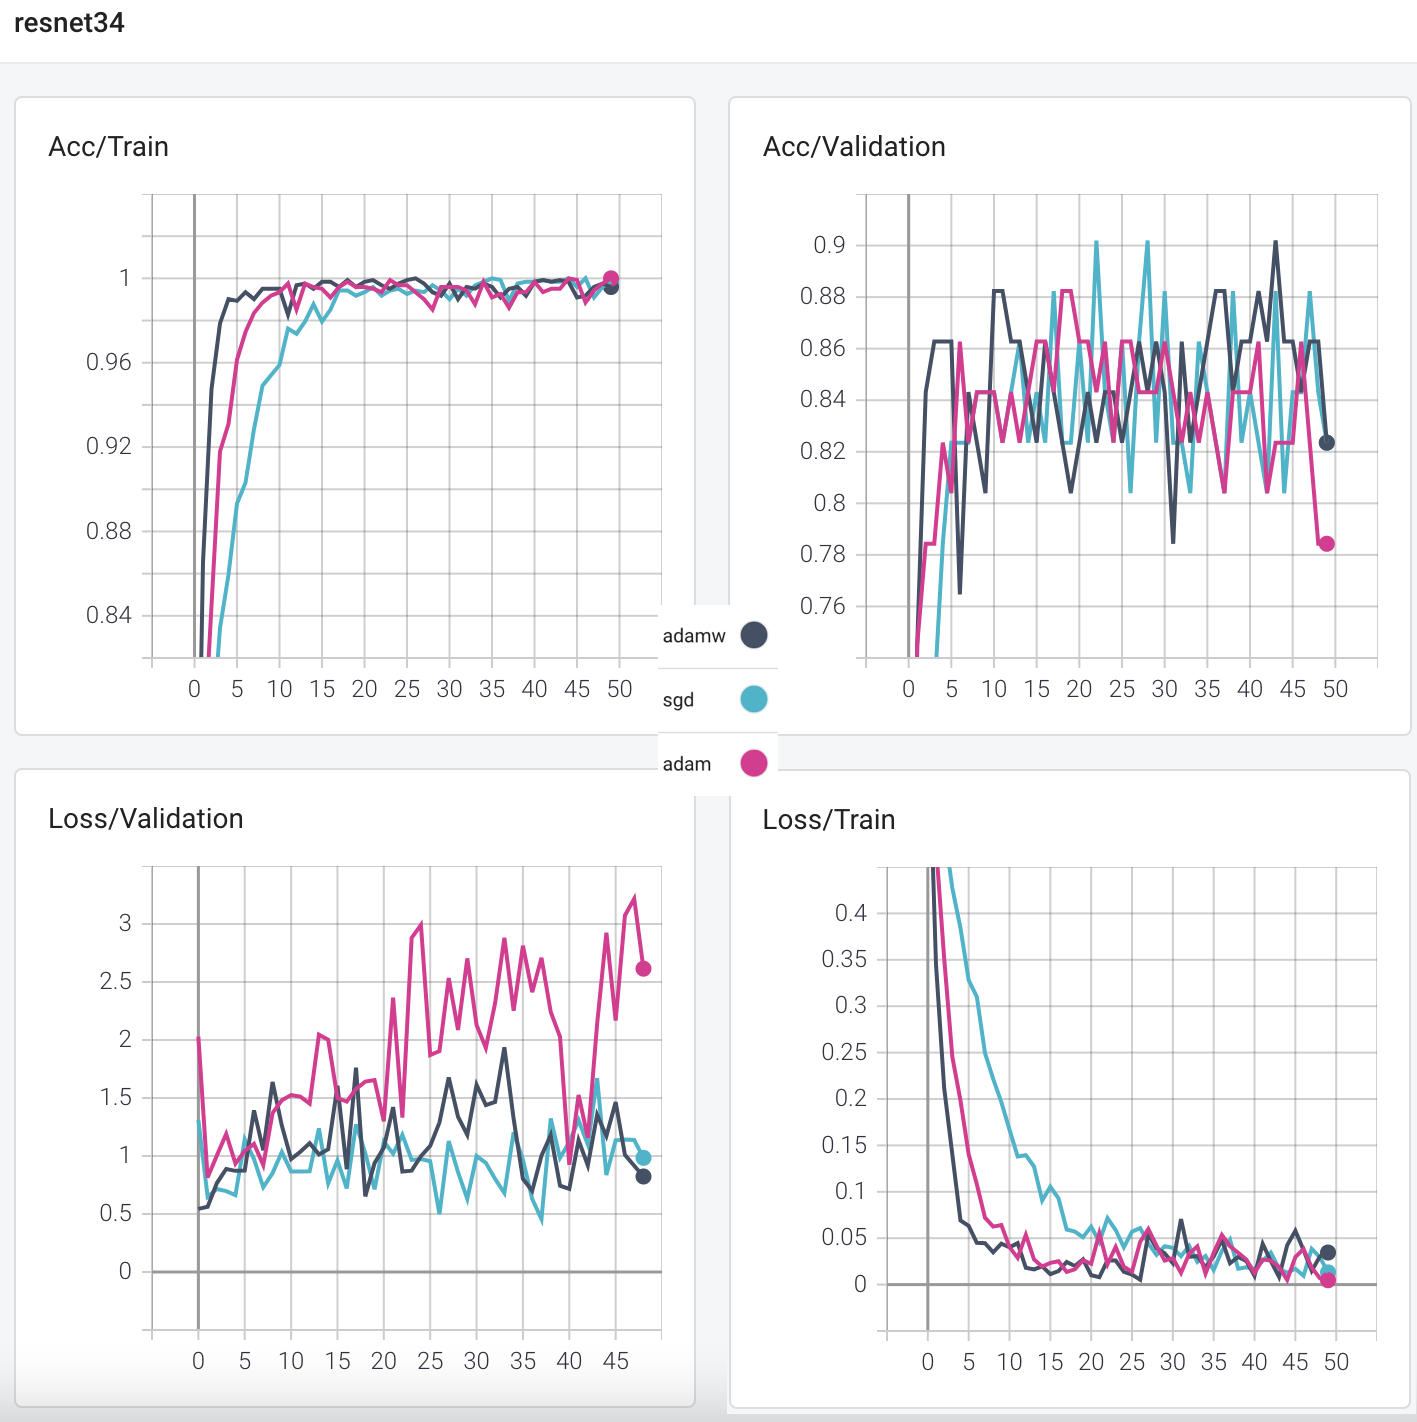
\includegraphics[width=\linewidth]{fig/resnet34.png}
    \vspace{2mm}
    \caption{ResNet-34 model accuracy and loss curves on train and validation processes with the SGD momentum, Adam, and AdamW optimizers.}
    \label{fig:resnet34_plots}
\end{figure}

\begin{figure}[!h]
    \centering
    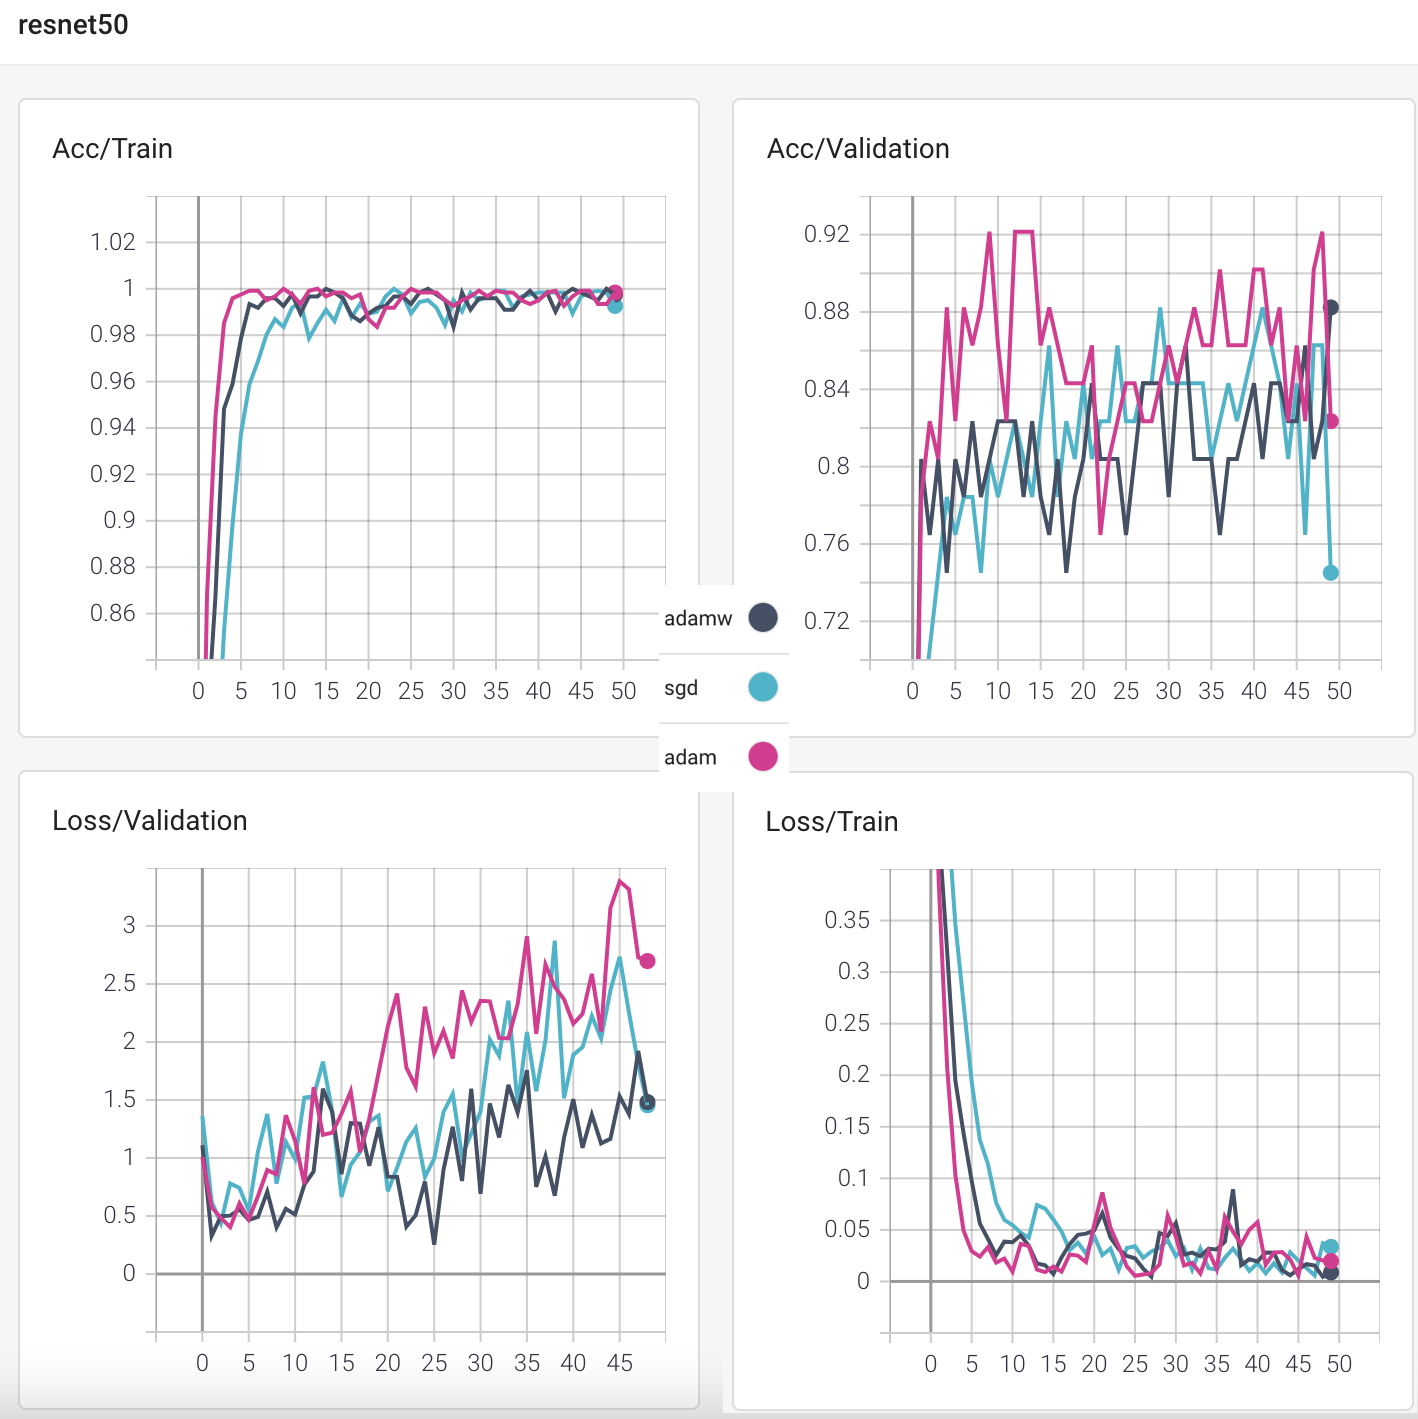
\includegraphics[width=\linewidth]{fig/resnet50.png}
    \vspace{2mm}
    \caption{ResNet-50 model accuracy and loss curves on train and validation processes with the SGD momentum, Adam, and AdamW optimizers.}
    \label{fig:resnet50_plots}
\end{figure}

\begin{figure}[!h]
    \centering
    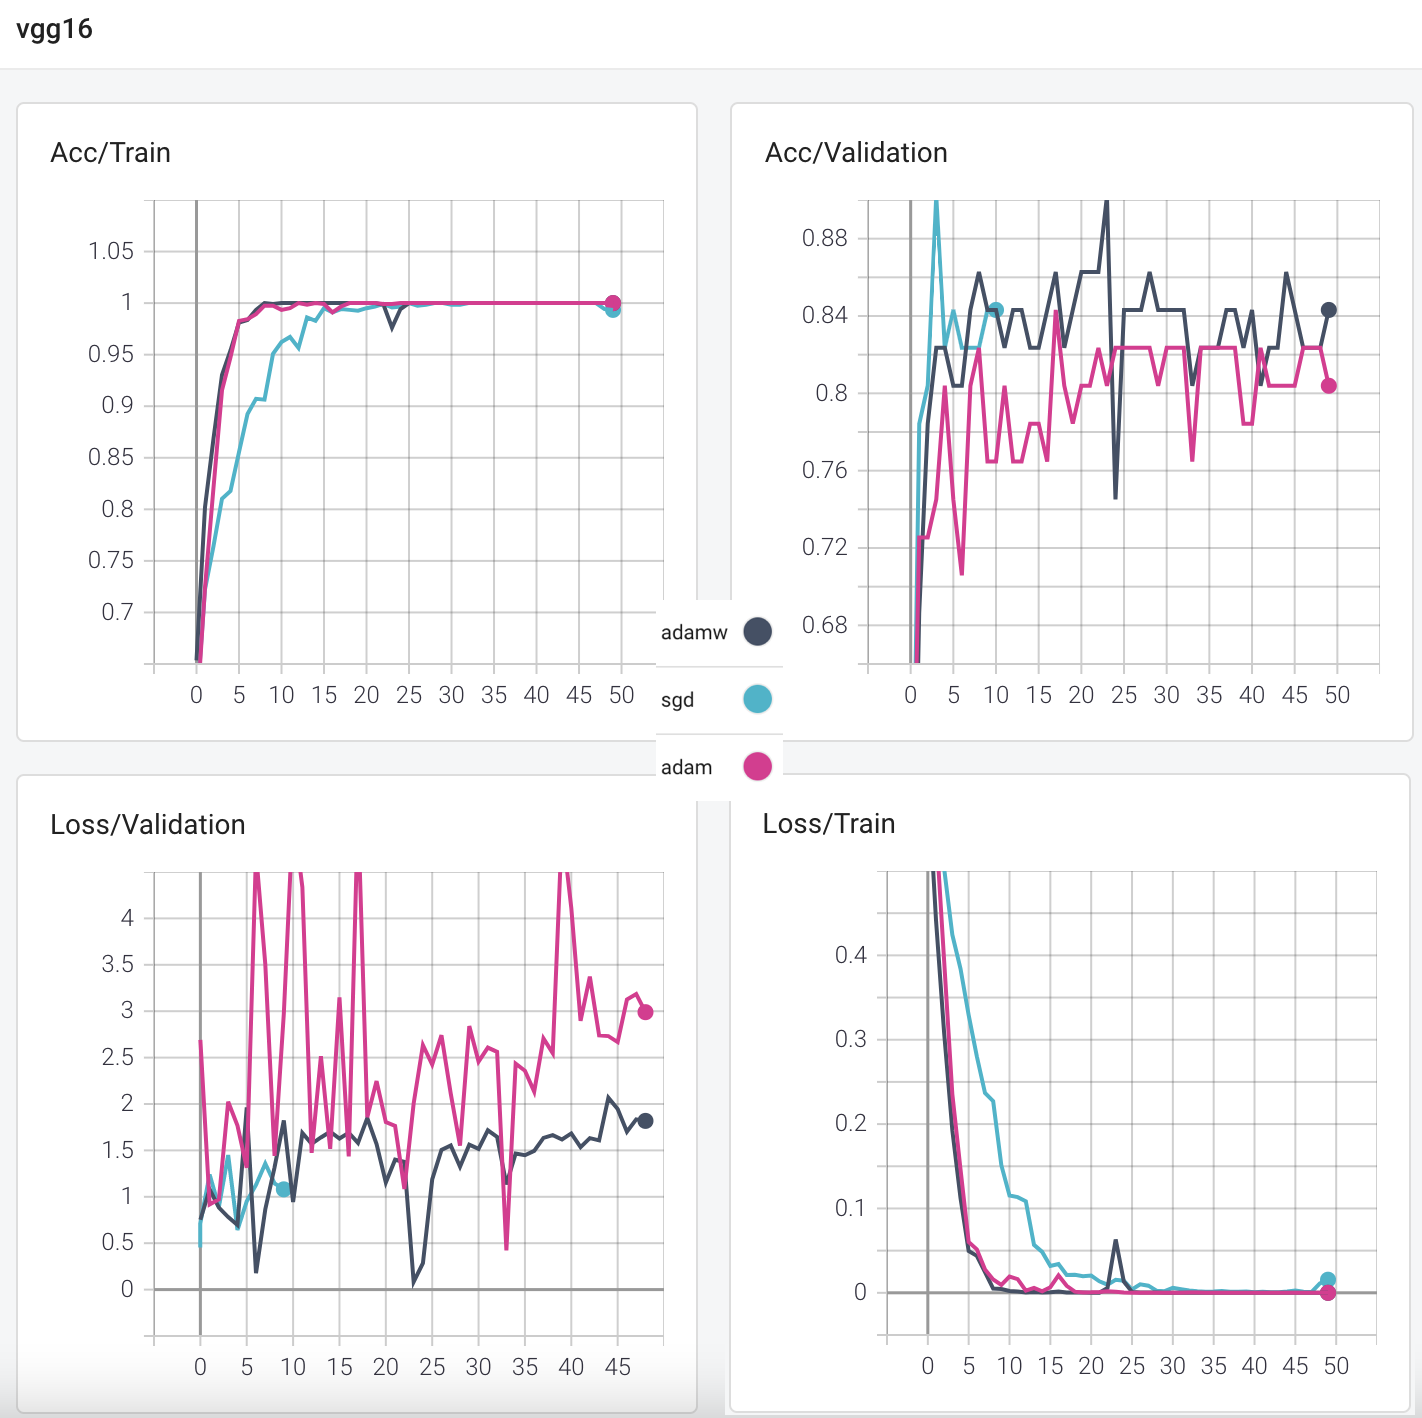
\includegraphics[width=\linewidth]{fig/vgg16.png}
    \vspace{2mm}
    \caption{VGG16 model accuracy and loss curves on train and validation processes for the SGD momentum, Adam, and AdamW optimizers.}
    \label{fig:vgg16_plots}
\end{figure}

\begin{figure}[!h]
    \centering
    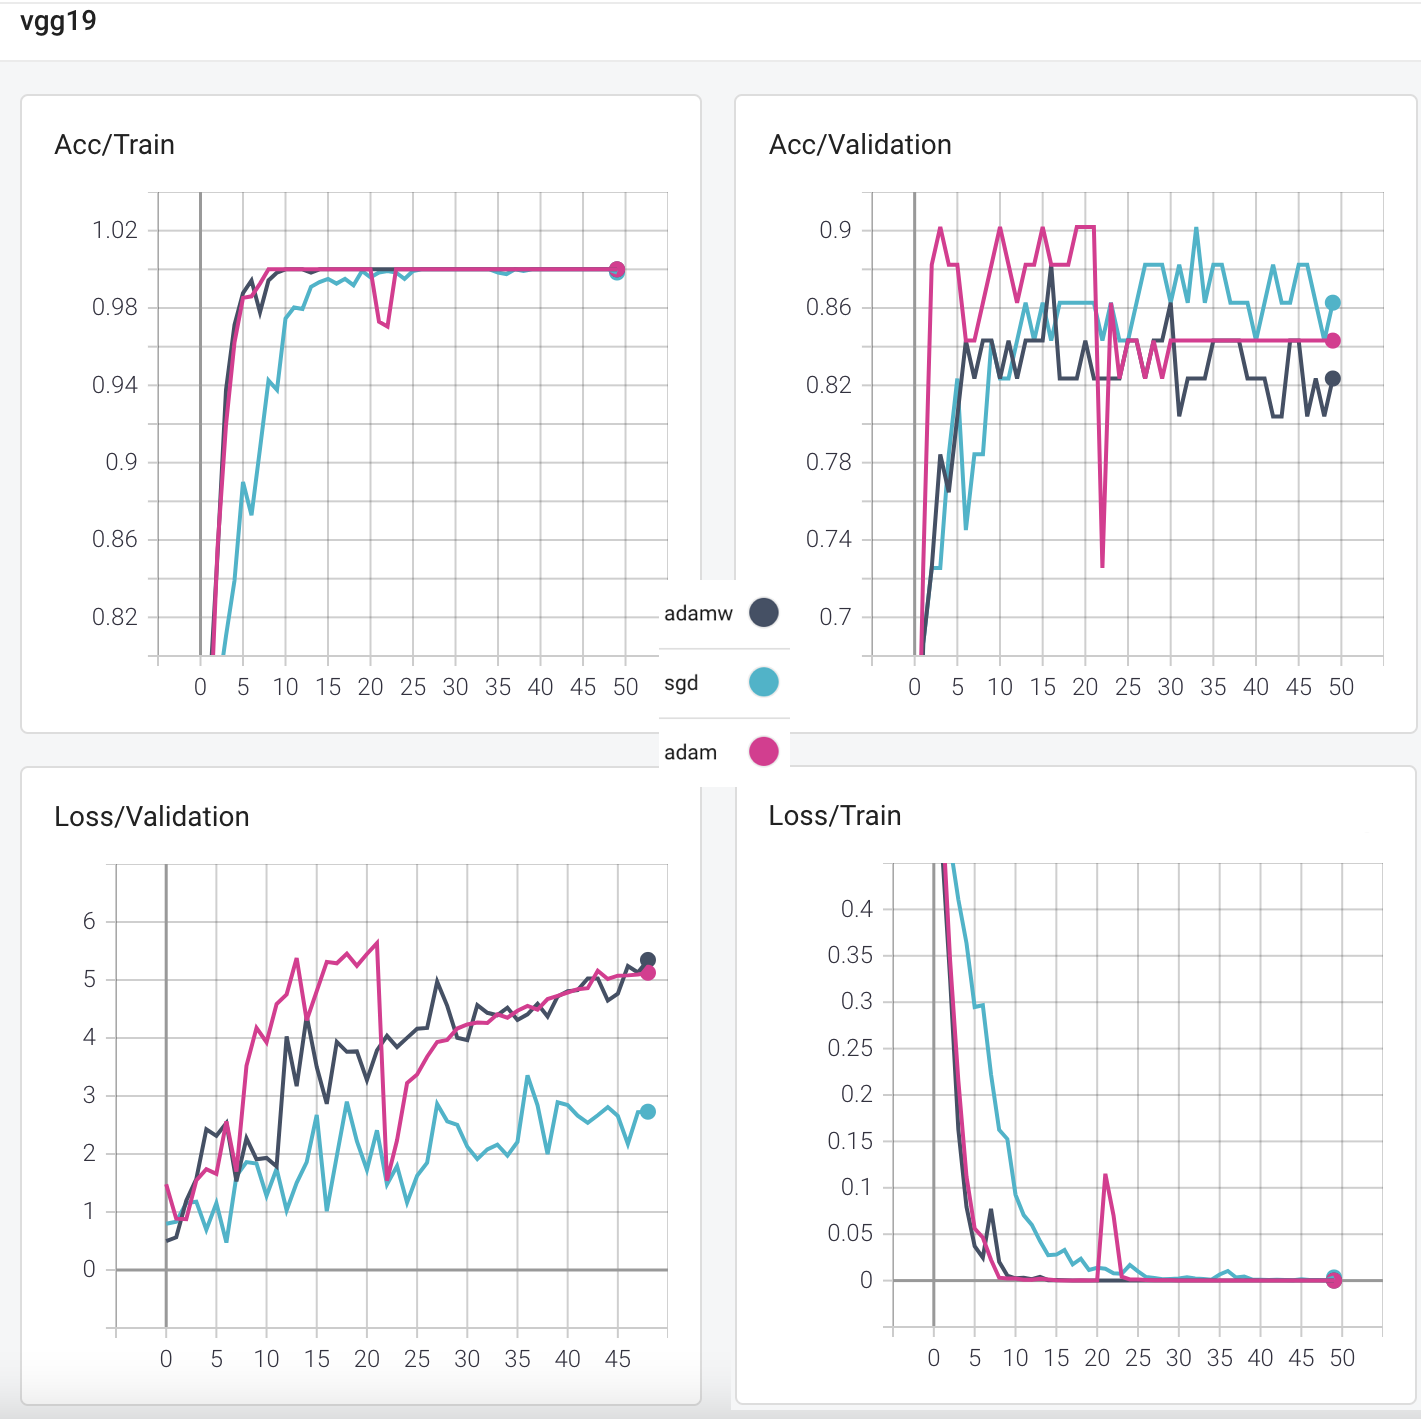
\includegraphics[width=\linewidth]{fig/vgg19.png}
    \vspace{2mm}
    \caption{VGG19 model accuracy and loss curves on train and validation processes for the SGD momentum, Adam, and AdamW optimizers.}
    \label{fig:vgg19_plots}
\end{figure}

% Please add the following required packages to your document preamble:
% \usepackage{multirow}
% \usepackage{lscape}
\begin{landscape}
\begin{table}[!h]
\centering
\caption{Comparison of results of AlexNet, ResNet-18, ResNet-34, ResNet-50, VGG16, and VGG19.}
\label{tab:cnn_result_table}
\begin{tabular}{c|l|cccccc|cc|c|c}
\hline
\multicolumn{2}{c|}{\textbf{Models and Optimizers}}  & \multicolumn{6}{c|}{\textbf{Metrics}}                                                                         & \multicolumn{2}{c|}{\textbf{Losses}}          & \multirow{2}{*}{\textbf{\begin{tabular}[c]{@{}c@{}}Last Train \\ Epoch\end{tabular}}} & \multirow{2}{*}{\textbf{\begin{tabular}[c]{@{}c@{}}Duration\\ (minutes)\end{tabular}}} \\ \cline{1-10}
\textbf{Model}                      & \multicolumn{1}{c|}{\textbf{Optimizer}}                   & \textbf{Accuracy (\%)} & \textbf{Sensitivity} & \textbf{Specificity} & \textbf{Precision} & \textbf{F1 Score} & \textbf{AUC Score} & \textbf{Last Train} & \textbf{Test} &                                                                                       &                                                                                        \\ \hline
\multirow{3}{*}{AlexNet}            & \begin{tabular}[c]{@{}l@{}}SGD\\ Momentum\end{tabular}    & 90.20                  & 0.9020               & 0.9026               & 0.9026             & 0.9020  & 0.9019          & 0.3503                   & 1.0316             & 35                                                                                    & 22                                                                                     \\
                                    & \begin{tabular}[c]{@{}l@{}}Adam\end{tabular} & 90.20                  & 0.9020               & 0.9011               & 0.9025             & 0.9019 & 0.9023           & 0.1265                   & 1.0373             & 8                                                                                     & 7                                                                                      \\
                                    & AdamW                                                     & 90.20                  & 0.9020               & 0.9042               & 0.9078             & 0.9017  & 0.9018               & 0.1549                   & 1.2347             & 9                                                                                     & 13                                                                                     \\ \hline
\multirow{3}{*}{ResNet-18}          & \begin{tabular}[c]{@{}l@{}}SGD\\ Momentum\end{tabular}    & 84.31                  & 0.8431               & 0.8430               & 0.8431             & 0.8431   & 0.8434         & 0.0194                   & 0.8252             & 29                                                                                    & 20                                                                                     \\
                                    & \begin{tabular}[c]{@{}l@{}}Adam\end{tabular} & 90.20                  & 0.9020               & 0.9026               & 0.9026             & 0.9020   & 0.9022         & 0.0288                   & 0.3631             & 43                                                                                    & 33                                                                                     \\
                                    & AdamW                                                     & 90.20                  & 0.9020               & 0.9042               & 0.9078             & 0.9020  & 0.9019           & 0.0171                   & 1.2423             & 16                                                                                    & 12                                                                                     \\ \hline
\multirow{3}{*}{ResNet-34}          & \begin{tabular}[c]{@{}l@{}}SGD\\ Momentum\end{tabular}    & 90.20                  & 0.9020               & 0.9026               & 0.9026             & 0.9020  & 0.9023          & 0.0460                   & 1.1830             & 22                                                                                    & 16                                                                                     \\
                                    & \begin{tabular}[c]{@{}l@{}}Adam\end{tabular} & 88.24                  & 0.8823               & 0.8838               & 0.8849             & 0.8823  & 0.8826          & 0.0136                   & 1.6412             & 18                                                                                    & 10                                                                                     \\
                                    & AdamW                                                     & 90.20                  & 0.9020               & 0.9026               & 0.9026             & 0.9020   & 0.9019         & 0.0253                   & 1.3553             & 43                                                                                    & 25                                                                                     \\ \hline
\multirow{3}{*}{\textbf{ResNet-50}} & \begin{tabular}[c]{@{}l@{}}SGD\\ Momentum\end{tabular}    & 88.24                  & 0.8823               & 0.8823               & 0.8823             & 0.8823  & 0.8821          & 0.0327                   & 1.2134             & 29                                                                                    & 14                                                                                     \\
                                    & \textbf{Adam}                                             & \textbf{92.16}         & \textbf{0.9216}      & \textbf{0.9215}      & \textbf{0.9216}    & \textbf{0.9216} & \textbf{0.9219}  & \textbf{0.0223}          & \textbf{1.3687}    & \textbf{9}                                                                                     & \textbf{7}                                                                                      \\
                                    & AdamW                                                     & 88.24                  & 0.8823               & 0.8823               & 0.8823             & 0.8823   & 0.8827         & 0.0260                   & 1.4826             & 50                                                                                    & 34                                                                                     \\ \hline
\multirow{3}{*}{VGG16}              & \begin{tabular}[c]{@{}l@{}}SGD\\ Momentum\end{tabular}    & 90.20                  & 0.9020               & 0.9042               & 0.9078             & 0.9017   & 0.9021         & 0.0318                   & 1.4500             & 15                                                                                    & 11                                                                                     \\
                                    & Adam                                                      & 84.31                  & 0.8431               & 0.8415               & 0.8450             & 0.8428   & 0.8432         & 0.0206                   & 5.1689             & 17                                                                                    & 15                                                                                     \\
                                    & AdamW                                                     & 90.20                  & 0.9020               & 0.8996               & 0.9074             & 0.9015   & 0.9023         & 0.0057                   & 0.0831             & 23                                                                                    & 19                                                                                     \\ \hline
\multirow{3}{*}{VGG19}              & \begin{tabular}[c]{@{}l@{}}SGD\\ Momentum\end{tabular}    & 90.20                  & 0.9020               & 0.9026               & 0.9026             & 0.9020     & 0.9020       & 0.0024                   & 2.1594             & 29                                                                                    & 26                                                                                     \\
                                    & \begin{tabular}[c]{@{}l@{}}Adam\end{tabular} & 90.20                  & 0.9020               & 0.9026               & 0.9026             & 0.9025    & 0.9019        & 0.0344                   & 1.5451             & 3                                                                                     & 2                                                                                      \\
                                    & AdamW                                                     & 88.24                  & 0.8823               & 0.8838               & 0.8849             & 0.8823    & 0.8825        & 0.0006                   & 2.8652             & 16                                                                                    & 15                                                                                     \\ \hline
\end{tabular}
\end{table}
\end{landscape}


For each CNN architecture, the best optimizer was detected according to its success on accuracy and loss values, and the confusion matrices for these CNN architecture and optimizer pairs were also reported in Tables \ref{tab:conf_alexnet}-\ref{tab:conf_vgg19}.
 
% Please add the following required packages to your document preamble:
% \usepackage{multirow}
\begin{table}[!h]
\centering
\caption{The confusion matrix of AlexNet model result with Adam optimizer.}
\label{tab:conf_alexnet}
\begin{tabular}{|cc|c|c|}
\cline{1-4}
                                                 &   & \multicolumn{2}{c|}{\textbf{Actual}} \\ \cline{3-4} 
                                                 &   & P            & N            \\ \hline
\multicolumn{1}{|c|}{\multirow{2}{*}{\textbf{Predicted}}} & P & 24           & 3            \\ \cline{2-4} 
\multicolumn{1}{|c|}{}                           & N & 2            & 22           \\ \hline
\end{tabular}
\end{table}

% Please add the following required packages to your document preamble:
% \usepackage{multirow}
\begin{table}[!h]
\centering
\caption{The confusion matrix of ResNet-18 model result with AdamW optimizer.}
\label{tab:conf_resnet18}
\begin{tabular}{|cc|c|c|}
\cline{1-4}
                                                 &   & \multicolumn{2}{c|}{\textbf{Actual}} \\ \cline{3-4} 
                                                 &   & P            & N            \\ \hline
\multicolumn{1}{|c|}{\multirow{2}{*}{\textbf{Predicted}}} & P & 22           & 1            \\ \cline{2-4} 
\multicolumn{1}{|c|}{}                           & N & 4            & 24           \\ \hline
\end{tabular}
\end{table}

% Please add the following required packages to your document preamble:
% \usepackage{multirow}
\begin{table}[!h]
\centering
\caption{The confusion matrix of ResNet-34 model result with AdamW optimizer.}
\label{tab:conf_resnet34}
\begin{tabular}{|cc|c|c|}
\cline{1-4}
                                                 &   & \multicolumn{2}{c|}{\textbf{Actual}} \\ \cline{3-4} 
                                                 &   & P            & N            \\ \hline
\multicolumn{1}{|c|}{\multirow{2}{*}{\textbf{Predicted}}} & P & 23           & 2            \\ \cline{2-4} 
\multicolumn{1}{|c|}{}                           & N & 3            & 23           \\ \hline
\end{tabular}
\end{table}

% Please add the following required packages to your document preamble:
% \usepackage{multirow}
\begin{table}[!h]
\centering
\caption{The confusion matrix of ResNet-50 model result with Adam optimizer.}
\label{tab:conf_resnet50}
\begin{tabular}{|cc|c|c|}
\cline{1-4}
                                                 &   & \multicolumn{2}{c|}{\textbf{Actual}} \\ \cline{3-4} 
                                                 &   & P            & N            \\ \hline
\multicolumn{1}{|c|}{\multirow{2}{*}{\textbf{Predicted}}} & P & 23           & 3            \\ \cline{2-4} 
\multicolumn{1}{|c|}{}                           & N & 2            & 23           \\ \hline
\end{tabular}
\end{table}

% Please add the following required packages to your document preamble:
% \usepackage{multirow}
\begin{table}[!h]
\centering
\caption{The confusion matrix of VGG16 model result with AdamW optimizer.}
\label{tab:conf_vgg16}
\begin{tabular}{|cc|c|c|}
\cline{1-4}
                                                 &   & \multicolumn{2}{c|}{\textbf{Actual}} \\ \cline{3-4} 
                                                 &   & P            & N            \\ \hline
\multicolumn{1}{|c|}{\multirow{2}{*}{\textbf{Predicted}}} & P & 25           & 4            \\ \cline{2-4} 
\multicolumn{1}{|c|}{}                           & N & 1            & 21           \\ \hline
\end{tabular}
\end{table}

% Please add the following required packages to your document preamble:
% \usepackage{multirow}
\begin{table}[!h]
\centering
\caption{The confusion matrix of VGG19 model result with SGD Momentum optimizer.}
\label{tab:conf_vgg19}
\begin{tabular}{|cc|c|c|}
\cline{1-4}
                                                 &   & \multicolumn{2}{c|}{\textbf{Actual}} \\ \cline{3-4} 
                                                 &   & P            & N            \\ \hline
\multicolumn{1}{|c|}{\multirow{2}{*}{\textbf{Predicted}}} & P & 23           & 2            \\ \cline{2-4} 
\multicolumn{1}{|c|}{}                           & N & 3            & 23           \\ \hline
\end{tabular}
\end{table}

\section{Machine Learning Results}



After the experiments of CNN models and obtaining the results, the deep feature sets were extracted from exactly the same train and test data. On the other side, the demographic information feature matrices were extracted for the same separation. In this section, we report the results for machine learning experiments on $X_{info}$, $X_{cnn}$ and $X_{all}$ defined in Section~\ref{sec:CH5_forming_features}.


 
\subsection{Results for $X_{info}$} \label{CH6:results_xinfo}

In Table~\ref{tab:ml_info_result_table}, the result for experimented machine learning algorithms with grid search on $X_{info}$ can be viewed. The reported results can be reproduced with the Python system seed as 4. The best results were obtained with KNN algorithm, and the final hyper-parameters can be seen on Table~\ref{tab:knn_info_params}. Furthermore, the confusion matrices are in Table~\ref{tab:knn_conf_matrix_xinfo}.

% Please add the following required packages to your document preamble:
% \usepackage{multirow}
\begin{table}[!h]
\centering
\caption{The results of machine learning experiments on demographic information.}
\label{tab:ml_info_result_table}
\begin{tabular}{cccc}
\hline
\multicolumn{2}{c}{} & \multicolumn{2}{c}{\textbf{Accuracy (\%)}}                                                                                                                                         \\ \cline{3-4}
\textbf{Model}            & \textbf{Regularizer}     & \textbf{\begin{tabular}[c]{@{}c@{}}Train Data\end{tabular}} & \textbf{\begin{tabular}[c]{@{}c@{}}Test Data\end{tabular}} \\ \hline \hline
\multirow{2}{*}{SVM}      & Lasso                    & 52.94                                                                                     & 52.94                                                                                    \\
                          & Ridge                    & 52.94                                                                                     & 52.94                                                                                    \\ \hline
\multirow{3}{*}{LR}       & -                        & 52.94                                                                                     & 52.94                                                                                    \\
                          & Lasso                    & 52.94                                                                                     & 52.94                                                                                    \\
                          & Ridge                    & 52.94                                                                                     & 52.94                                                                                    \\ \hline
\textbf{KNN}                       & \textbf{-}                        &\textbf{ 56.86  }                                                                                   & \textbf{56.86}                                                                                    \\ \hline
\multirow{2}{*}{LDA}      & -                        & 52.94                                                                                     & 52.94                                                                                    \\
                          & Lasso                    & 52.94                                                                                     & 52.94                                                    \\ \hline                                
\end{tabular}
\end{table}

\begin{table}[!h]
\centering
\caption{KNN algorithm hyper-parameters for $X_{info}$.}
\label{tab:knn_info_params}
\begin{tabular}{lcc}
\hline
\multicolumn{1}{c}{\textbf{Hyper-Parameter}} & \textbf{\begin{tabular}[c]{@{}c@{}}Train Data\end{tabular}} & \textbf{\begin{tabular}[c]{@{}c@{}}Test Data\end{tabular}} \\ \hline \hline
Number of Neighbors                          & 17                                                                                        & 17                                                                                       \\
Type of Majority Voting                      & uniform                                                                                   & uniform                                                                                  \\
Neighborhood Finder                          & brute force                                                                               & brute force                                                                              \\
Metric  Function                            & euclidean                                                                                 & euclidean       \\ \hline                                                                         
\end{tabular}
\end{table}

\begin{table}[!h]
\centering
\caption{Confusion matrices for KNN experiments on demographic information.}
\label{tab:knn_conf_matrix_xinfo}
\begin{tabular}{|cc|c|c|c|c|}
\cline{1-6}
                                                          &   & \multicolumn{4}{c|}{\textbf{Actual}}                                                                                                                                                                                       \\ \cline{3-6} 
                                                          &   & \multicolumn{2}{c|}{\textbf{Train Data}} & \multicolumn{2}{c|}{\textbf{Test Data}} \\ \cline{3-6} 
                                                          &   & \text{\:\:} P \text{\:\:}                                                   & N                                                    & \text{\:} P \text{\:}                                                   & N                                                   \\ \hline
\multicolumn{1}{|c|}{\multirow{2}{*}{\textbf{Predicted}}} & P & 5                                                     & 1                                                    & 5                                                     & 1                                                   \\ \cline{2-6} 
\multicolumn{1}{|c|}{}                                    & N & 21                                                    & 24                                                   & 21                                                    & 24                                                  \\ \hline
\end{tabular}
\end{table}

\subsection{Results for $X_{cnn}$} \label{CH6:results_xcnn}

In Table~\ref{tab:ml_cnn_result_table}, the machine learning experiments with grid search on different $X_{cnn}$ feature matrices obtained from AlexNet model with Adam optimizer, ResNet-18 model AdamW optimizer, ResNet-34 model AdamW optimizer, ResNet-50 model with Adam optimizer, VGG16 model with AdamW optimizer, and VGG19 model SGD optimizer can be seen. The reported results can be reproduced with the Python system seed as 4.

\textcolor{purple}{Since all final results of models were yielded in both train data by using cross-validation, and test data in a directly testing method, all tables referenced here includes the results both for train data and test data. The reason why we experimented in both ways is to see the generalized performance of models, and the performance of models specific to our test data. Further information can be found in Section~\ref{CH5:train_test_ml} and Section~\ref{ch:CH7}.}

\textcolor{purple}{Since the best performance was reached by ResNet-50 model together with Adam optimizer, here we reported the outputs for this combination.} The final hyper-parameters for $X_{cnn\_ResNet50}$ feature matrix constructed by the help of ResNet-50 model Adam optimizer can be seen in Tables \ref{tab:svmridge_cnn_params}-\ref{tab:ldalasso_cnn_params}. Furthermore, the confusion matrices and all other metrics derived from these confusion matrices are given in Tables \ref{tab:svmridge_cnn_results}-\ref{tab:ldalasso_cnn_results}.

\textcolor{purple}{It can be seen in Table~\ref{tab:ml_cnn_result_table} that we obtained the highest metrics on the feature matrix $X_{cnn}$ extracted by using the weights ResNet-50 model together with Adam optimizer, as we obtained the higher result by ResNet-50 model with Adam optimizer during the CNN experiments. Therefore, we reported the detailed result tables for the $X_{cnn\_ResNet50}$ feature matrix constructed by the help of this CNN weights. It can be seen from these reports embedded in Tables \ref{tab:svmridge_cnn_results}-\ref{tab:ldalasso_cnn_results} that the results obtained on test data is clearly higher than the results obtained on train data. On the other hand, we cannot state the best one; however, the worst results were obtained by LDA algorithm both for test and train data performances. The given hyper-parameters given in Tables \ref{tab:svmridge_cnn_params}-\ref{tab:ldalasso_cnn_params} can be used for reproducibility of our work.}

% Please add the following required packages to your document preamble:
% \usepackage{multirow}
% \usepackage{graphicx}
\begin{landscape}
\begin{table}[]
\centering
\caption{The results of machine learning experiments on $X_{cnn}$. }
\label{tab:ml_cnn_result_table}
\resizebox{1.8\textwidth}{!}{%
\begin{tabular}{cc|cccccccccccc}
\hline
\multicolumn{2}{c|}{\textbf{}}                   & \multicolumn{12}{c}{\textbf{Accuracy (\%)}}                                                                           \\ \hline
\multirow{2}{*}{\textbf{Model}} & \multirow{2}{*}{\textbf{Regularizer}} & \multicolumn{6}{c|}{\textbf{Train Data}}                                                                                                                                                                                                                                                                                                                                                                                    & \multicolumn{6}{c}{\textbf{Test Data}}                                                                                                                                                                                                                                                                                                                                                                  \\ \cline{3-14} 
                                &                                       & \textbf{\begin{tabular}[c]{@{}c@{}}AlexNet\\ (Adam)\end{tabular}} & \textbf{\begin{tabular}[c]{@{}c@{}}ResNet-18\\ (AdamW)\end{tabular}} & \textbf{\begin{tabular}[c]{@{}c@{}}ResNet-34\\ (AdamW)\end{tabular}} & \textbf{\begin{tabular}[c]{@{}c@{}}ResNet-50\\ (Adam)\end{tabular}} & \textbf{\begin{tabular}[c]{@{}c@{}}VGG16\\ (AdamW)\end{tabular}} & \multicolumn{1}{c|}{\textbf{\begin{tabular}[c]{@{}c@{}}VGG19\\ (SGD Momentum)\end{tabular}}} & \textbf{\begin{tabular}[c]{@{}c@{}}AlexNet\\ (Adam)\end{tabular}} & \textbf{\begin{tabular}[c]{@{}c@{}}ResNet-18\\ (AdamW)\end{tabular}} & \textbf{\begin{tabular}[c]{@{}c@{}}ResNet-34\\ (AdamW)\end{tabular}} & \textbf{\begin{tabular}[c]{@{}c@{}}ResNet-50\\ (Adam)\end{tabular}} & \textbf{\begin{tabular}[c]{@{}c@{}}VGG16\\ (AdamW)\end{tabular}} & \textbf{\begin{tabular}[c]{@{}c@{}}VGG19\\ (SGD Momentum)\end{tabular}} \\ \hline \hline
\multirow{2}{*}{SVM}           
                                & Lasso                                 & 90.20                                                             & 90.20                                                                & 84.31                                                                & 86.27                                                               & 88.24                                                            & \multicolumn{1}{c|}{86.27}                                                                   & 90.20                                                             & 90.20                                                                & 90.20                                                                & 92.16                                                               & 88.24                                                            & 88.24                                                                   \\ 
                                 & Ridge                                 & 88.24                                                             & 88.24                                                                & 90.20                                                                & 92.16                                                               & 88.24                                                            & \multicolumn{1}{c|}{88.24}                                                                   & 90.20                                                             & 88.24                                                                & 90.20                                                                & 92.16                                                               & 88.24                                                            & 90.20                                                                   \\ \hline
\multirow{3}{*}{LR}             & -                                     & 90.20                                                             & 88.24                                                                & 90.20                                                                & 92.16                                                               & 90.20                                                            & \multicolumn{1}{c|}{90.20}                                                                   & 90.20                                                             & 88.24                                                                & 90.20                                                                & 92.16                                                               & 90.20                                                            & 90.20                                                                   \\
                               
                                & Lasso                                 & 84.31                                                             & 86.27                                                                & 84.31                                                                & 86.27                                                               & 86.27                                                            & \multicolumn{1}{c|}{84.31}                                                                   & 88.24                                                             & 86.27                                                                & 90.20                                                                & 92.16                                                               & 86.27                                                            & 86.27                                                                   \\ 
                                 & Ridge                                 & 90.20                                                             & 88.24                                                                & 90.20                                                                & 92.16                                                               & 88.24                                                            & \multicolumn{1}{c|}{88.24}                                                                   & 90.20                                                             & 88.24                                                                & 90.20                                                                & 92.16                                                               & 88.24                                                            & 88.24                                                                   \\ \hline
KNN                             & -                                     & 88.24                                                             & 88.24                                                                & 90.20                                                                & 92.16                                                               & 86.27                                                            & \multicolumn{1}{c|}{90.20}                                                                   & 90.20                                                             & 88.24                                                                & 90.20                                                                & 92.16                                                               & 86.27                                                            & 90.20                                                                   \\ \hline
\multirow{2}{*}{LDA}            & -                                     & 82.35                                                             & 82.35                                                                & 82.35                                                                & 84.31                                                               & 82.35                                                            & \multicolumn{1}{c|}{84.31}                                                                   & 84.31                                                             & 84.31                                                                & 82.35                                                                & 84.31                                                               & 84.31                                                            & 84.31                                                                   \\
                                & Lasso                                 & 88.24                                                             & 88.24                                                                & 88.24                                                                & 90.20                                                               & 88.24                                                            & \multicolumn{1}{c|}{88.24}                                                                   & 90.20                                                             & 90.20                                                                & 90.20                                                                & 92.16                                                               & 88.24                                                            & 90.20                                                                   \\ \hline
\end{tabular}%
}
\end{table}
\end{landscape}

\begin{table}[!h]
\centering
\caption{The tuned hyper-parameters of SVM algorithm with Lasso penalty on $X_{cnn\_ResNet50}$.}
\label{tab:svmlasso_cnn_params}
\begin{tabular}{lcc}
\hline
\multicolumn{1}{c}{\textbf{Hyper-Parameter}} & \textbf{\begin{tabular}[c]{@{}c@{}} Train Data\end{tabular}} & \textbf{\begin{tabular}[c]{@{}c@{}}Test Data\end{tabular}} \\ \hline \hline
Regularization Parameter                     & 5e-3                                                                                      & 5e-2        \\ \hline                                                                             
\end{tabular}
\end{table}

\begin{table}[!h]
\centering
\caption{The tuned hyper-parameters of SVM algorithm with Ridge penalty on $X_{cnn\_ResNet50}$.}
\label{tab:svmridge_cnn_params}
\begin{tabular}{lcc}
\hline
\multicolumn{1}{c}{\textbf{Hyper-Parameter}} & \textbf{\begin{tabular}[c]{@{}c@{}}Train Data\end{tabular}} & \textbf{\begin{tabular}[c]{@{}c@{}}Test Data\end{tabular}} \\ \hline \hline
Kernel Function                              & linear                                                                                    & linear                                                                                   \\
Regularization Parameter                     & 5e-5                                                                                      & 5e-5  \\ \hline                                                                                  
\end{tabular}
\end{table}



\begin{table}[!h]
\centering
\caption{The tuned hyper-parameters of LR algorithm on $X_{cnn\_ResNet50}$.}
\label{tab:lr_cnn_params}
\begin{tabular}{lcc}
\hline
\multicolumn{1}{c}{\textbf{Hyper-Parameter}} & \textbf{\begin{tabular}[c]{@{}c@{}} Train Data\end{tabular}} & \textbf{\begin{tabular}[c]{@{}c@{}}Test Data\end{tabular}} \\ \hline \hline
Solver Function                              & newton-cg                                                                                 & newton-cg    \\ \hline                                                                            
\end{tabular}
\end{table}



\begin{table}[!h]
\centering
\caption{The tuned hyper-parameters of LR algorithm wit Lasso penalty for $X_{cnn\_ResNet50}$.}
\label{tab:lrlasso_cnn_params}
\begin{tabular}{lcc}
\hline
\multicolumn{1}{c}{\textbf{Hyper-Parameter}} & \textbf{\begin{tabular}[c]{@{}c@{}}Train Data\end{tabular}} & \textbf{\begin{tabular}[c]{@{}c@{}}Test Data\end{tabular}} \\ \hline \hline
Solver Function                              & liblinear                                                                                 & liblinear                                                                                \\
Regularization Parameter                     & 2e-2                                                                                      & 1.0    \\ \hline                                                                                  
\end{tabular}
\end{table}

\begin{table}[!h]
\centering
\caption{The tuned hyper-parameters of LR algorithm with Ridge penalty on $X_{cnn\_ResNet50}$.}
\label{tab:lrridge_cnn_params}
\begin{tabular}{lcc}
\hline
\multicolumn{1}{c}{\textbf{Hyper-Parameter}} & \textbf{\begin{tabular}[c]{@{}c@{}}Train Data\end{tabular}} & \textbf{\begin{tabular}[c]{@{}c@{}}Test Data\end{tabular}} \\ \hline \hline
Solver Function                              & liblinear                                                                                 & liblinear                                                                                \\
Regularization Parameter                     & 5e-5                                                                                     & 5e-5     \\ \hline                                                                               
\end{tabular}
\end{table}

\begin{table}[!h]
\centering
\caption{The tuned hyper-parameters of KNN algorithm on $X_{cnn\_ResNet50}$.}
\label{tab:knn_cnn_params}
\begin{tabular}{lcc}
\hline
\multicolumn{1}{c}{\textbf{Hyper-Parameter}} & \textbf{\begin{tabular}[c]{@{}c@{}} Train Data\end{tabular}} & \textbf{\begin{tabular}[c]{@{}c@{}}Test Data\end{tabular}} \\ \hline \hline
Number of Neighbors                          & 3                                                                                         & 3                                                                                        \\
Type of Majority Voting                      & uniform                                                                                   & uniform                                                                                  \\
Neighborhood Finder                          & ball tree                                                                                 & ball tree                                                                                \\
Metric Function                              & euclidean                                                                                 & euclidean   \\ \hline                                                                             
\end{tabular}
\end{table}

\begin{table}[!h]
\centering
\caption{The tuned hyper-parameters of LDA algorithm  on $X_{cnn\_ResNet50}$.}
\label{tab:lda_cnn_params}
\begin{tabular}{lcc}
\hline
\multicolumn{1}{c}{\textbf{Hyper-Parameter}}                                                                & \textbf{\begin{tabular}[c]{@{}c@{}}Train Data\end{tabular}} & \textbf{\begin{tabular}[c]{@{}c@{}}Test Data\end{tabular}} \\ \hline \hline
Solver Function                                                                                             & svd                                                                                       & svd                                                                                      \\
\begin{tabular}[c]{@{}l@{}}Computing the Weighted\\ Within-Class Covariance\\ (for svd solver)\end{tabular} & True                                                                                      & True        \\ \hline                                                                             
\end{tabular}
\end{table}

\begin{table}[!h]
\centering
\caption{The tuned hyper-parameters of LDA algorithm with Lasso penalty  for $X_{cnn\_ResNet50}$.}
\label{tab:ldalasso_cnn_params}
\begin{tabular}{lcc}
\hline
\multicolumn{1}{c}{\textbf{Hyper-Parameter}} & \textbf{\begin{tabular}[c]{@{}c@{}}Train Data\end{tabular}} & \textbf{\begin{tabular}[c]{@{}c@{}}Test Data\end{tabular}} \\ \hline \hline
Regularization Parameter                     & 5e-5                                                                                      & 5e-3    \\ \hline                                                                                 
\end{tabular}
\end{table}

% Please add the following required packages to your document preamble:
% \usepackage{multirow}
% \usepackage{graphicx}
% \usepackage{lscape}
\begin{landscape}

% Please add the following required packages to your document preamble:
% \usepackage{multirow}
% \usepackage{graphicx}
\begin{table}[!h]
\centering
\caption{The confusion matrices and results obtained by SVM algorithm with Lasso penalty for $X_{cnn\_ResNet50}$.}
\label{tab:svmlasso_cnn_results}
\resizebox{1.8\textwidth}{!}{%
\begin{tabular}{cc|c|c|cccccc|c|c|cccccc}
\cline{3-18}
                                                          &   & \multicolumn{8}{c|}{\textbf{Train Data}}                                                                                                        & \multicolumn{8}{c|}{\textbf{Test Data}}                                                                                                                              \\ \cline{3-18} 
                                                          &   & \multicolumn{2}{c|}{\textbf{Actual}} & \textbf{Accuracy (\%)} & \textbf{Sensitivity} & \textbf{Specificity} & \textbf{Precision} & \textbf{F1 Score} & \textbf{AUC Score} & \multicolumn{2}{c|}{\textbf{Actual}} & \textbf{Accuracy (\%)} & \textbf{Sensitivity} & \textbf{Specificity} & \textbf{Precision} & \textbf{F1 Score} & \multicolumn{1}{c|}{\textbf{AUC Score}} \\ \cline{3-18} 
                                                          &   & P                 & N                & 86.27                  & 0.8627               & 0.8665               & 0.8777             & 0.8617            & 0.8646             & P                 & N                & 92.16                  & 0.9216               & 0.9230               & 0.9243             & 0.9215            & \multicolumn{1}{c|}{0.9223}             \\ \hline
\multicolumn{1}{|c|}{\multirow{2}{*}{\textbf{Predicted}}} & P & 20                & 1                &                        &                      &                      &                    &                   &                    & 23                & 1                &                        &                      &                      &                    &                   &                                         \\ \cline{2-4} \cline{11-12}
\multicolumn{1}{|c|}{}                                    & N & 6                 & 24               &                        &                      &                      &                    &                   &                    & 3                 & 24               &                        &                      &                      &                    &                   &                                         \\ \cline{1-4} \cline{11-12}  
\end{tabular}%
}
\end{table}

\begin{table}[!h]
\centering
\caption{The confusion matrices and results obtained by SVM algorithm with Ridge penalty on $X_{cnn\_ResNet50}$.}
\label{tab:svmridge_cnn_results}
\resizebox{1.8\textwidth}{!}{%
\begin{tabular}{cc|c|c|cccccc|c|c|cccccc}
\cline{3-18}
                                                          &   & \multicolumn{8}{c|}{\textbf{Train Data}}                                                                                                        & \multicolumn{8}{c|}{\textbf{Test Data}}                                                                                                                              \\ \cline{3-18} 
                                                          &   & \multicolumn{2}{c|}{\textbf{Actual}} & \textbf{Accuracy (\%)} & \textbf{Sensitivity} & \textbf{Specificity} & \textbf{Precision} & \textbf{F1 Score} & \textbf{AUC Score} & \multicolumn{2}{c|}{\textbf{Actual}} & \textbf{Accuracy (\%)} & \textbf{Sensitivity} & \textbf{Specificity} & \textbf{Precision} & \textbf{F1 Score} & \multicolumn{1}{c|}{\textbf{AUC Score}} \\ \cline{3-18} 
                                                          &   & P                 & N                & 92.16                  & 0.9216               & 0.9230               & 0.9243             & 0.9215            & 0.9223             & P                 & N                & 92.16                  & 0.9216               & 0.9230               & 0.9243             & 0.9215            & \multicolumn{1}{c|}{0.9223}             \\ \hline
\multicolumn{1}{|c|}{\multirow{2}{*}{\textbf{Predicted}}} & P & 23                & 1                &                        &                      &                      &                    &                   &                    & 23                & 1                &                        &                      &                      &                    &                   &                                         \\ \cline{2-4} \cline{11-12}
\multicolumn{1}{|c|}{}                                    & N & 3                 & 24               &                        &                      &                      &                    &                   &                    & 3                 & 24               &                        &                      &                      &                    &                   &                                         \\ \cline{1-4} \cline{11-12} 
\end{tabular}%
}
\end{table}



% Please add the following required packages to your document preamble:
% \usepackage{multirow}
% \usepackage{graphicx}
\begin{table}[!h]
\centering
\caption{The confusion matrices and results obtained by LR algorithm for $X_{cnn\_ResNet50}$.}
\label{tab:lr_cnn_results}
\resizebox{1.8\textwidth}{!}{%
\begin{tabular}{cc|c|c|cccccc|c|c|cccccc}
\cline{3-18}
                                                          &   & \multicolumn{8}{c|}{\textbf{Train Data}}                                                                                                        & \multicolumn{8}{c|}{\textbf{Test Data}}                                                                                                                              \\ \cline{3-18} 
                                                          &   & \multicolumn{2}{c|}{\textbf{Actual}} & \textbf{Accuracy (\%)} & \textbf{Sensitivity} & \textbf{Specificity} & \textbf{Precision} & \textbf{F1 Score} & \textbf{AUC Score} & \multicolumn{2}{c|}{\textbf{Actual}} & \textbf{Accuracy (\%)} & \textbf{Sensitivity} & \textbf{Specificity} & \textbf{Precision} & \textbf{F1 Score} & \multicolumn{1}{c|}{\textbf{AUC Score}} \\ \cline{3-18} 
                                                          &   & P                 & N                & 92.16                  & 0.9216               & 0.9230               & 0.9243             & 0.9215            & 0.9223             & P                 & N                & 92.16                  & 0.9216               & 0.9230               & 0.9243             & 0.9215            & \multicolumn{1}{c|}{0.9223}             \\ \hline
\multicolumn{1}{|c|}{\multirow{2}{*}{\textbf{Predicted}}} & P & 23                & 1                &                        &                      &                      &                    &                   &                    & 23                & 1                &                        &                      &                      &                    &                   &                                         \\ \cline{2-4} \cline{11-12}
\multicolumn{1}{|c|}{}                                    & N & 3                 & 24               &                        &                      &                      &                    &                   &                    & 3                 & 24               &                        &                      &                      &                    &                   &                                         \\ \cline{1-4} \cline{11-12}  
\end{tabular}%
}
\end{table}

\begin{table}[!h]
\centering
\caption{The confusion matrices and results obtained by LR algorithm with Lasso penalty on $X_{cnn\_ResNet50}$.}
\label{tab:lrlasso_cnn_results}
\resizebox{1.8\textwidth}{!}{%
\begin{tabular}{cc|c|c|cccccc|c|c|cccccc}
\cline{3-18}
                                                          &   & \multicolumn{8}{c|}{\textbf{Train Data}}                                                                                                        & \multicolumn{8}{c|}{\textbf{Test Data}}                                                                                                                              \\ \cline{3-18} 
                                                          &   & \multicolumn{2}{c|}{\textbf{Actual}} & \textbf{Accuracy (\%)} & \textbf{Sensitivity} & \textbf{Specificity} & \textbf{Precision} & \textbf{F1 Score} & \textbf{AUC Score} & \multicolumn{2}{c|}{\textbf{Actual}} & \textbf{Accuracy (\%)} & \textbf{Sensitivity} & \textbf{Specificity} & \textbf{Precision} & \textbf{F1 Score} & \multicolumn{1}{c|}{\textbf{AUC Score}} \\ \cline{3-18} 
                                                          &   & P                 & N                & 86.27                  & 0.8627               & 0.8665               & 0.8777             & 0.8617            & 0.8646             & P                 & N                & 92.16                  & 0.9216               & 0.9230               & 0.9243             & 0.9215            & \multicolumn{1}{c|}{0.9223}             \\ \hline
\multicolumn{1}{|c|}{\multirow{2}{*}{\textbf{Predicted}}} & P & 20                & 1                &                        &                      &                      &                    &                   &                    & 23                & 1                &                        &                      &                      &                    &                   &                                         \\ \cline{2-4} \cline{11-12}
\multicolumn{1}{|c|}{}                                    & N & 6                 & 24               &                        &                      &                      &                    &                   &                    & 3                 & 24               &                        &                      &                      &                    &                   &                                         \\ \cline{1-4} \cline{11-12}  
\end{tabular}%
}
\end{table}


% Please add the following required packages to your document preamble:
% \usepackage{multirow}
% \usepackage{graphicx}
\begin{table}[!h]
\centering
\caption{The confusion matrices and results obtained by LR algorithm with Ridge penalty on $X_{cnn\_ResNet50}$.}
\label{tab:lrridge_cnn_results}
\resizebox{1.8\textwidth}{!}{%
\begin{tabular}{cc|c|c|cccccc|c|c|cccccc}
\cline{3-18}
                                                          &   & \multicolumn{8}{c|}{\textbf{Result for Grid Search on Train Data}}                                                                                                        & \multicolumn{8}{c|}{\textbf{Result for Grid Search on Test Data}}                                                                                                                              \\ \cline{3-18} 
                                                          &   & \multicolumn{2}{c|}{\textbf{Actual}} & \textbf{Accuracy (\%)} & \textbf{Sensitivity} & \textbf{Specificity} & \textbf{Precision} & \textbf{F1 Score} & \textbf{AUC Score} & \multicolumn{2}{c|}{\textbf{Actual}} & \textbf{Accuracy (\%)} & \textbf{Sensitivity} & \textbf{Specificity} & \textbf{Precision} & \textbf{F1 Score} & \multicolumn{1}{c|}{\textbf{AUC Score}} \\ \cline{3-18} 
                                                          &   & P                 & N                & 92.16                  & 0.9216               & 0.9230               & 0.9243             & 0.9215            & 0.9223             & P                 & N                & 92.16                  & 0.9216               & 0.9230               & 0.9243             & 0.9215            & \multicolumn{1}{c|}{0.9223}             \\ \hline
\multicolumn{1}{|c|}{\multirow{2}{*}{\textbf{Predicted}}} & P & 23                & 1                &                        &                      &                      &                    &                   &                    & 23                & 1                &                        &                      &                      &                    &                   &                                         \\ \cline{2-4} \cline{11-12}
\multicolumn{1}{|c|}{}                                    & N & 3                 & 24               &                        &                      &                      &                    &                   &                    & 3                 & 24               &                        &                      &                      &                    &                   &                                         \\ \cline{1-4} \cline{11-12}  
\end{tabular}%
}
\end{table}

% Please add the following required packages to your document preamble:
% \usepackage{multirow}
% \usepackage{graphicx}

% Please add the following required packages to your document preamble:
% \usepackage{multirow}
% \usepackage{graphicx}
\begin{table}[!h]
\centering
\caption{The confusion matrices and results obtained by KNN algorithm on $X_{cnn\_ResNet50}$.}
\label{tab:knn_cnn_results}
\resizebox{1.8\textwidth}{!}{%
\begin{tabular}{cc|c|c|cccccc|c|c|cccccc}
\cline{3-18}
                                                          &   & \multicolumn{8}{c|}{\textbf{Train Data}}                                                                                                        & \multicolumn{8}{c|}{\textbf{Test Data}}                                                                                                                              \\ \cline{3-18} 
                                                          &   & \multicolumn{2}{c|}{\textbf{Actual}} & \textbf{Accuracy (\%)} & \textbf{Sensitivity} & \textbf{Specificity} & \textbf{Precision} & \textbf{F1 Score} & \textbf{AUC Score} & \multicolumn{2}{c|}{\textbf{Actual}} & \textbf{Accuracy (\%)} & \textbf{Sensitivity} & \textbf{Specificity} & \textbf{Precision} & \textbf{F1 Score} & \multicolumn{1}{c|}{\textbf{AUC Score}} \\ \cline{3-18} 
                                                          &   & P                 & N                & 92.16                  & 0.9216               & 0.9230               & 0.9243             & 0.9215            & 0.9223             & P                 & N                & 92.16                  & 0.9216               & 0.9230               & 0.9243             & 0.9215            & \multicolumn{1}{c|}{0.9223}             \\ \hline
\multicolumn{1}{|c|}{\multirow{2}{*}{\textbf{Predicted}}} & P & 23                & 1                &                        &                      &                      &                    &                   &                    & 23                & 1                &                        &                      &                      &                    &                   &                                         \\ \cline{2-4} \cline{11-12}
\multicolumn{1}{|c|}{}                                    & N & 3                 & 24               &                        &                      &                      &                    &                   &                    & 3                 & 24               &                        &                      &                      &                    &                   &                                         \\ \cline{1-4} \cline{11-12}  
\end{tabular}%
}
\end{table}

% Please add the following required packages to your document preamble:
% \usepackage{multirow}
% \usepackage{graphicx}
\begin{table}[!h]
\centering
\caption{The confusion matrices and results obtained by LDA algorithm on $X_{cnn\_ResNet50}$.}
\label{tab:lda_cnn_results}
\resizebox{1.8\textwidth}{!}{%
\begin{tabular}{cc|c|c|cccccc|c|c|cccccc}
\cline{3-18}
                                                          &   & \multicolumn{8}{c|}{\textbf{Train Data}}                                                                                                        & \multicolumn{8}{c|}{\textbf{Test Data}}                                                                                                                              \\ \cline{3-18} 
                                                          &   & \multicolumn{2}{c|}{\textbf{Actual}} & \textbf{Accuracy (\%)} & \textbf{Sensitivity} & \textbf{Specificity} & \textbf{Precision} & \textbf{F1 Score} & \textbf{AUC Score} & \multicolumn{2}{c|}{\textbf{Actual}} & \textbf{Accuracy (\%)} & \textbf{Sensitivity} & \textbf{Specificity} & \textbf{Precision} & \textbf{F1 Score} & \multicolumn{1}{c|}{\textbf{AUC Score}} \\ \cline{3-18} 
                                                          &   & P                 & N                & 84.31                  & 0.8431               & 0.8476               & 0.8638             & 0.8413            & 0.8454             & P                 & N                & 84.31                  & 0.8431               & 0.8476               & 0.8638             & 0.8413            & \multicolumn{1}{c|}{0.8454}             \\ \hline
\multicolumn{1}{|c|}{\multirow{2}{*}{\textbf{Predicted}}} & P & 19                & 1                &                        &                      &                      &                    &                   &                    & 19                & 1                &                        &                      &                      &                    &                   &                                         \\ \cline{2-4} \cline{11-12}
\multicolumn{1}{|c|}{}                                    & N & 7                 & 24               &                        &                      &                      &                    &                   &                    & 7                 & 24               &                        &                      &                      &                    &                   &                                         \\ \cline{1-4} \cline{11-12} 
\end{tabular}%
}
\end{table}

% Please add the following required packages to your document preamble:
% \usepackage{multirow}
% \usepackage{graphicx}
\begin{table}[!h]
\centering
\caption{The confusion matrices and results obtained by LDA algorithm with Lasso penalty on $X_{cnn\_ResNet50}$.}
\label{tab:ldalasso_cnn_results}
\resizebox{1.8\textwidth}{!}{%
\begin{tabular}{cc|c|c|cccccc|c|c|cccccc}
\cline{3-18}
                                                          &   & \multicolumn{8}{c|}{\textbf{Train Data}}                                                                                                        & \multicolumn{8}{c|}{\textbf{Test Data}}                                                                                                                              \\ \cline{3-18} 
                                                          &   & \multicolumn{2}{c|}{\textbf{Actual}} & \textbf{Accuracy (\%)} & \textbf{Sensitivity} & \textbf{Specificity} & \textbf{Precision} & \textbf{F1 Score} & \textbf{AUC Score} & \multicolumn{2}{c|}{\textbf{Actual}} & \textbf{Accuracy (\%)} & \textbf{Sensitivity} & \textbf{Specificity} & \textbf{Precision} & \textbf{F1 Score} & \multicolumn{1}{c|}{\textbf{AUC Score}} \\ \cline{3-18} 
                                                          &   & P                 & N                & 90.20                  & 0.9020               & 0.9042               & 0.9078             & 0.9017            & 0.9045             & P                 & N                & 92.16                  & 0.9216               & 0.9230               & 0.9243             & 0.9215            & \multicolumn{1}{c|}{0.9223}             \\ \hline
\multicolumn{1}{|c|}{\multirow{2}{*}{\textbf{Predicted}}} & P & 22                & 1                &                        &                      &                      &                    &                   &                    & 23                & 1                &                        &                      &                      &                    &                   &                                         \\ \cline{2-4} \cline{11-12}
\multicolumn{1}{|c|}{}                                    & N & 4                 & 24               &                        &                      &                      &                    &                   &                    & 3                 & 24               &                        &                      &                      &                    &                   &                                         \\ \cline{1-4} \cline{11-12}  
\end{tabular}%
}
\end{table}

\end{landscape}

\subsection{Results for $X_{all}$} \label{CH6:results_xall}

In Table~\ref{tab:ml_all_result_table}, the machine learning experiments with grid search on different $X_{all}$ feature matrices obtained from AlexNet model with Adam optimizer, ResNet-18 model AdamW optimizer, ResNet-34 model AdamW optimizer, ResNet-50 model with Adam optimizer, VGG16 model with AdamW optimizer, and VGG19 model SGD optimizer can be seen. The reported results can be reproduced with Python system seed as 4. 

\textcolor{purple}{Since all final results of models were yielded in both train data by using cross-validation, and test data in a directly testing method, all tables referenced here includes the results both for train data and test data. The reason why we experimented in both ways is to see the generalized performance of models, and the performance of models specific to our test data. Further information can be found in Section~\ref{CH5:train_test_ml} and Section~\ref{ch:CH7}.}

\textcolor{purple}{Since the best performance was reached by ResNet-50 model together with Adam optimizer, here we reported the outputs for this combination.} The final hyper-parameters for $X_{all\_ResNet50}$ feature matrix constructed by the help of ResNet-50 model Adam optimizer can be seen in Tables \ref{tab:svmridge_all_params}-\ref{tab:ldalasso_all_params}. Furthermore, the confusion matrices and all other metrics derived from these confusion matrices are on Tables \ref{tab:svmridge_all_results}-\ref{tab:ldalasso_all_results}.

\textcolor{purple}{It can be seen in Table~\ref{tab:ml_all_result_table} that we obtained the highest metrics on the feature matrix $X_{all}$ extracted by using the weights ResNet-50 model together with Adam optimizer, as we obtained the higher result by ResNet-50 model with Adam optimizer during the CNN experiments. Therefore, we reported the detailed result tables for the $X_{all\_ResNet50}$ feature matrix constructed by the help of this CNN weights. It can be seen from these reports embedded in Tables \ref{tab:svmridge_all_results}-\ref{tab:ldalasso_all_results} that the results obtained on test data is clearly higher than the results obtained on train data. On the other hand, we cannot state the best one; however, the worst results were obtained by LDA algorithm both for test and train data performances. The given hyper-parameters given in Tables \ref{tab:svmridge_all_params}-\ref{tab:ldalasso_all_params} can be used for reproducibility of our work.}


% Please add the following required packages to your document preamble:
% \usepackage{multirow}
% \usepackage{graphicx}
% \usepackage{lscape}
\begin{landscape}
\begin{table}[]
\centering
\caption{The results of machine learning experiments on $X_{all}$.}
\label{tab:ml_all_result_table}
\resizebox{1.8\textwidth}{!}{%
\begin{tabular}{cc|clllllclllll}
\hline
\multicolumn{2}{c|}{\textbf{}}                   & \multicolumn{12}{c}{\textbf{Accuracy (\%)}}                                                                                                                                                                                                                                                                                                                                                                                                                                                                                                                                                                                                                                                                                                                                                                                                                                                                                                                                                                                                                                    \\ \hline
\multirow{2}{*}{\textbf{Model}} & \multirow{2}{*}{\textbf{Regularizer}} & \multicolumn{6}{c|}{\textbf{Train Data}}                                                                                                                                                                                                                                                                                                                                                                                                                                                                    & \multicolumn{6}{c}{\textbf{Test Data}}                                                                                                                                                                                                                                                                                                                                                                                                                                                                      \\ \cline{3-14} 
                                &                                       & \textbf{\begin{tabular}[c]{@{}c@{}}AlexNet\\ (Adam)\end{tabular}} & \multicolumn{1}{c}{\textbf{\begin{tabular}[c]{@{}c@{}}ResNet-18\\ (AdamW)\end{tabular}}} & \multicolumn{1}{c}{\textbf{\begin{tabular}[c]{@{}c@{}}ResNet-34\\ (AdamW)\end{tabular}}} & \multicolumn{1}{c}{\textbf{\begin{tabular}[c]{@{}c@{}}ResNet-50\\ (Adam)\end{tabular}}} & \multicolumn{1}{c}{\textbf{\begin{tabular}[c]{@{}c@{}}VGG16\\ (AdamW)\end{tabular}}} & \multicolumn{1}{c|}{\textbf{\begin{tabular}[c]{@{}c@{}}VGG19\\ (SGD Momentum)\end{tabular}}} & \textbf{\begin{tabular}[c]{@{}c@{}}AlexNet\\ (Adam)\end{tabular}} & \multicolumn{1}{c}{\textbf{\begin{tabular}[c]{@{}c@{}}ResNet-18\\ (AdamW)\end{tabular}}} & \multicolumn{1}{c}{\textbf{\begin{tabular}[c]{@{}c@{}}ResNet-34\\ (AdamW)\end{tabular}}} & \multicolumn{1}{c}{\textbf{\begin{tabular}[c]{@{}c@{}}ResNet-50\\ (Adam)\end{tabular}}} & \multicolumn{1}{c}{\textbf{\begin{tabular}[c]{@{}c@{}}VGG16\\ (AdamW)\end{tabular}}} & \multicolumn{1}{c}{\textbf{\begin{tabular}[c]{@{}c@{}}VGG19\\ (SGD Momentum)\end{tabular}}} \\ \hline \hline
\multirow{2}{*}{SVM}            
                                & Lasso                                 & 90.20                                                             & 90.20                                                                & 84.31                                                                & 86.27                                                               & 88.24                                                            & \multicolumn{1}{c|}{86.27}                                                                   & 90.20                                                             & 90.20                                                                & 90.20                                                                & 92.16                                                               & 88.24                                                            & 88.24                                                                   \\ 
                                & Ridge                                 & 88.24                                                             & 90.20                                                                & 90.20                                                                & 92.16                                                               & 88.24                                                            & \multicolumn{1}{c|}{88.24}                                                                   & 90.20                                                             & 88.24                                                                & 90.20                                                                & 92.16                                                               & 88.24                                                            & 90.20                                                                   \\ \hline
\multirow{3}{*}{LR}             & -                                     & 90.20                                                             & 88.24                                                                & 90.20                                                                & 92.16                                                               & 90.20                                                            & \multicolumn{1}{c|}{90.20}                                                                   & 90.20                                                             & 88.24                                                                & 90.20                                                                & 92.16                                                               & 90.20                                                            & 90.20                                                                   \\
                               
                                & Lasso                                 & 84.31                                                             & 86.27                                                                & 84.31                                                                & 88.24                                                               & 86.27                                                            & \multicolumn{1}{c|}{86.27}                                                                   & 88.24                                                             & 86.27                                                                & 90.20                                                                & 92.16                                                               & 86.27                                                            & 88.24                                                                   \\ 
                                 & Ridge                                 & 90.20                                                             & 88.24                                                                & 90.20                                                                & 92.16                                                               & 88.24                                                            & \multicolumn{1}{c|}{88.24}                                                                   & 90.20                                                             & 88.24                                                                & 90.20                                                                & 92.16                                                               & 88.24                                                            & 88.24                                                                   \\ \hline
KNN                             & -                                     & 90.20                                                             & 88.24                                                                & 90.20                                                                & 92.16                                                               & 86.27                                                            & \multicolumn{1}{c|}{90.20}                                                                   & 90.20                                                             & 88.24                                                                & 90.20                                                                & 92.16                                                               & 86.27                                                            & 90.20                                                                   \\ \hline
\multirow{2}{*}{LDA}            & -                                     & 82.35                                                             & 82.35                                                                & 82.35                                                                & 84.31                                                               & 82.35                                                            & \multicolumn{1}{c|}{84.31}                                                                   & 84.31                                                             & 84.31                                                                & 82.35                                                                & 84.31                                                               & 84.31                                                            & 84.31                                                                   \\
                                & Lasso                                 & 88.24                                                             & 88.24                                                                & 88.24                                                                & 90.20                                                               & 88.24                                                            & \multicolumn{1}{c|}{88.24}                                                                   & 90.20                                                             & 90.20                                                                & 90.20                                                                & 92.16                                                               & 88.24                                                            & 90.20                                                                   \\ \hline
\end{tabular}%
}
\end{table}
\end{landscape}



\begin{table}[!h]
\centering
\caption{The tuned hyper-parameters of SVM algorithm with Lasso penalty on $X_{all\_ResNet50}$.}
\label{tab:svmlasso_all_params}
\begin{tabular}{lcc}
\hline
\multicolumn{1}{c}{\textbf{Hyper-Parameter}} & \textbf{\begin{tabular}[c]{@{}c@{}} Train Data\end{tabular}} & \textbf{\begin{tabular}[c]{@{}c@{}}Test Data\end{tabular}} \\ \hline \hline
Regularization Parameter                     & 5e-3                                                                                      & 5e-2   \\ \hline                                                                                 
\end{tabular}
\end{table}

\begin{table}[!h]
\centering
\caption{The tuned hyper-parameters of SVM algorithm with Ridge penalty on $X_{all\_ResNet50}$.}
\label{tab:svmridge_all_params}
\begin{tabular}{lcc}
\hline
\multicolumn{1}{c}{\textbf{Hyper-Parameter}} & \textbf{\begin{tabular}[c]{@{}c@{}}Train Data\end{tabular}} & \textbf{\begin{tabular}[c]{@{}c@{}}Test Data\end{tabular}} \\ \hline \hline
Kernel Function                              & linear                                                                                    & linear                                                                                   \\
Regularization Parameter                     & 5e-5                                                                                      & 5e-5  \\ \hline                                                                                  
\end{tabular}
\end{table}

\begin{table}[!h]
\centering
\caption{The tuned hyper-parameters of LR algorithm on $X_{all\_ResNet50}$.}
\label{tab:lr_all_params}
\begin{tabular}{lcc}
\hline
\multicolumn{1}{c}{\textbf{Hyper-Parameter}} & \textbf{\begin{tabular}[c]{@{}c@{}} Train Data\end{tabular}} & \textbf{\begin{tabular}[c]{@{}c@{}}Test Data\end{tabular}} \\ \hline \hline
Solver Function                              & newton-cg                                                                                 & newton-cg  \\ \hline                                                                             
\end{tabular}
\end{table}



\begin{table}[!h]
\centering
\caption{The tuned hyper-parameters of LR algorithm with Lasso on $X_{all\_ResNet50}$.}
\label{tab:lrlasso_all_params}
\begin{tabular}{lcc}
\hline
\multicolumn{1}{c}{\textbf{Hyper-Parameter}} & \textbf{\begin{tabular}[c]{@{}c@{}} Train Data\end{tabular}} & \textbf{\begin{tabular}[c]{@{}c@{}}Test Data\end{tabular}} \\ \hline \hline
Solver Function                              & liblinear                                                                                 & liblinear                                                                                \\
Regularization Parameter                     & 2e-2                                                                                      & 2.0  \\ \hline                                                                                   
\end{tabular}
\end{table}

\begin{table}[!h]
\centering
\caption{The tuned hyper-parameters of LR algorithm with Ridge penalty on $X_{all\_ResNet50}$.}
\label{tab:lrridge_all_params}
\begin{tabular}{lcc}
\hline
\multicolumn{1}{c}{\textbf{Hyper-Parameter}} & \textbf{\begin{tabular}[c]{@{}c@{}} Train Data\end{tabular}} & \textbf{\begin{tabular}[c]{@{}c@{}}Test Data\end{tabular}} \\ \hline \hline
Solver Function                              & liblinear                                                                                 & liblinear                                                                                \\
Regularization Parameter                     & 5e-5                                                                                     & 5e-5   \\ \hline                                                                                
\end{tabular}
\end{table}

\begin{table}[!h]
\centering
\caption{The tuned hyper-parameters of KNN algorithm on $X_{all\_ResNet50}$.}
\label{tab:knn_all_params}
\begin{tabular}{lcc}
\hline
\multicolumn{1}{c}{\textbf{Hyper-Parameter}} & \textbf{\begin{tabular}[c]{@{}c@{}} Train Data\end{tabular}} & \textbf{\begin{tabular}[c]{@{}c@{}}Test Data\end{tabular}} \\ \hline \hline
Number of Neighbors                          & 3                                                                                         & 3                                                                                        \\
Type of Majority Voting                      & uniform                                                                                   & uniform                                                                                  \\
Neighborhood Finder                          & ball tree                                                                                 & ball tree                                                                                \\
Metric Function                              & euclidean                                                                                 & euclidean  \\ \hline                                                                             
\end{tabular}
\end{table}

\begin{table}[!h]
\centering
\caption{The tuned hyper-parameters of LDA algorithm on $X_{all\_ResNet50}$.}
\label{tab:lda_all_params}
\begin{tabular}{lcc}
\hline
\multicolumn{1}{c}{\textbf{Hyper-Parameter}}                                                                & \textbf{\begin{tabular}[c]{@{}c@{}} Train Data\end{tabular}} & \textbf{\begin{tabular}[c]{@{}c@{}}Test Data\end{tabular}} \\ \hline \hline
Solver Function                                                                                             & svd                                                                                       & svd                                                                                      \\
\begin{tabular}[c]{@{}l@{}}Computing the Weighted\\ Within-Class Covariance\\ (for svd solver)\end{tabular} & True                                                                                      & True   \\ \hline                                                                                 
\end{tabular}
\end{table}

\begin{table}[!h]
\centering
\caption{The tuned hyper-parameters of LDA algorithm with Lasso penalty on $X_{all\_ResNet50}$.}
\label{tab:ldalasso_all_params}
\begin{tabular}{lcc}
\hline
\multicolumn{1}{c}{\textbf{Hyper-Parameter}} & \textbf{\begin{tabular}[c]{@{}c@{}} Train Data\end{tabular}} & \textbf{\begin{tabular}[c]{@{}c@{}}Test Data\end{tabular}} \\ \hline \hline
Regularization Parameter                     & 5e-5                                                                                      & 5e-3   \\ \hline                                                                                 
\end{tabular}
\end{table}

% Please add the following required packages to your document preamble:
% \usepackage{multirow}
% \usepackage{graphicx}
% \usepackage{lscape}
\begin{landscape}

% Please add the following required packages to your document preamble:
% \usepackage{multirow}
% \usepackage{graphicx}
\begin{table}[!h]
\centering
\caption{The confusion matrices and results obtained by SVM algorithm with Lasso penalty on $X_{all\_ResNet50}$.}
\label{tab:svmlasso_all_results}
\resizebox{1.8\textwidth}{!}{%
\begin{tabular}{cc|c|c|cccccc|c|c|cccccc}
\cline{3-18}
                                                          &   & \multicolumn{8}{c|}{\textbf{Train Data}}                                                                                                        & \multicolumn{8}{c|}{\textbf{Test Data}}                                                                                                                              \\ \cline{3-18} 
                                                          &   & \multicolumn{2}{c|}{\textbf{Actual}} & \textbf{Accuracy (\%)} & \textbf{Sensitivity} & \textbf{Specificity} & \textbf{Precision} & \textbf{F1 Score} & \textbf{AUC Score} & \multicolumn{2}{c|}{\textbf{Actual}} & \textbf{Accuracy (\%)} & \textbf{Sensitivity} & \textbf{Specificity} & \textbf{Precision} & \textbf{F1 Score} & \multicolumn{1}{c|}{\textbf{AUC Score}} \\ \cline{3-18} 
                                                          &   & P                 & N                & 86.27                  & 0.8627               & 0.8665               & 0.8777             & 0.8617            & 0.8646             & P                 & N                & 92.16                  & 0.9216               & 0.9230               & 0.9243             & 0.9215            & \multicolumn{1}{c|}{0.9223}             \\ \hline
\multicolumn{1}{|c|}{\multirow{2}{*}{\textbf{Predicted}}} & P & 20                & 1                &                        &                      &                      &                    &                   &                    & 23                & 1                &                        &                      &                      &                    &                   &                                         \\ \cline{2-4} \cline{11-12}
\multicolumn{1}{|c|}{}                                    & N & 6                 & 24               &                        &                      &                      &                    &                   &                    & 3                 & 24               &                        &                      &                      &                    &                   &                                         \\ \cline{1-4} \cline{11-12}
\end{tabular}%
}
\end{table}

\begin{table}[!h]
\centering
\caption{The confusion matrices and results obtained by SVM algorithm with Ridge penalty on $X_{all\_ResNet50}$.}
\label{tab:svmridge_all_results}
\resizebox{1.8\textwidth}{!}{%
\begin{tabular}{cc|c|c|cccccc|c|c|cccccc}
\cline{3-18}
                                                          &   & \multicolumn{8}{c|}{\textbf{Train Data}}                                                                                                        & \multicolumn{8}{c|}{\textbf{Test Data}}                                                                                                                              \\ \cline{3-18} 
                                                          &   & \multicolumn{2}{c|}{\textbf{Actual}} & \textbf{Accuracy (\%)} & \textbf{Sensitivity} & \textbf{Specificity} & \textbf{Precision} & \textbf{F1 Score} & \textbf{AUC Score} & \multicolumn{2}{c|}{\textbf{Actual}} & \textbf{Accuracy (\%)} & \textbf{Sensitivity} & \textbf{Specificity} & \textbf{Precision} & \textbf{F1 Score} & \multicolumn{1}{c|}{\textbf{AUC Score}} \\ \cline{3-18} 
                                                          &   & P                 & N                & 92.16                  & 0.9216               & 0.9230               & 0.9243             & 0.9215            & 0.9223             & P                 & N                & 92.16                  & 0.9216               & 0.9230               & 0.9243             & 0.9215            & \multicolumn{1}{c|}{0.9223}             \\ \hline
\multicolumn{1}{|c|}{\multirow{2}{*}{\textbf{Predicted}}} & P & 23                & 1                &                        &                      &                      &                    &                   &                    & 23                & 1                &                        &                      &                      &                    &                   &                                         \\ \cline{2-4} \cline{11-12}
\multicolumn{1}{|c|}{}                                    & N & 3                 & 24               &                        &                      &                      &                    &                   &                    & 3                 & 24               &                        &                      &                      &                    &                   &                                         \\ \cline{1-4} \cline{11-12}
\end{tabular}%
}
\end{table}


% Please add the following required packages to your document preamble:
% \usepackage{multirow}
% \usepackage{graphicx}
\begin{table}[!h]
\centering
\caption{The confusion matrices and results obtained by LR algorithm on $X_{all\_ResNet50}$.}
\label{tab:lr_all_results}
\resizebox{1.8\textwidth}{!}{%
\begin{tabular}{cc|c|c|cccccc|c|c|cccccc}
\cline{3-18}
                                                          &   & \multicolumn{8}{c|}{\textbf{Train Data}}                                                                                                        & \multicolumn{8}{c|}{\textbf{Test Data}}                                                                                                                              \\ \cline{3-18} 
                                                          &   & \multicolumn{2}{c|}{\textbf{Actual}} & \textbf{Accuracy (\%)} & \textbf{Sensitivity} & \textbf{Specificity} & \textbf{Precision} & \textbf{F1 Score} & \textbf{AUC Score} & \multicolumn{2}{c|}{\textbf{Actual}} & \textbf{Accuracy (\%)} & \textbf{Sensitivity} & \textbf{Specificity} & \textbf{Precision} & \textbf{F1 Score} & \multicolumn{1}{c|}{\textbf{AUC Score}} \\ \cline{3-18} 
                                                          &   & P                 & N                & 92.16                  & 0.9216               & 0.9230               & 0.9243             & 0.9215            & 0.9223             & P                 & N                & 92.16                  & 0.9216               & 0.9230               & 0.9243             & 0.9215            & \multicolumn{1}{c|}{0.9223}             \\ \hline
\multicolumn{1}{|c|}{\multirow{2}{*}{\textbf{Predicted}}} & P & 23                & 1                &                        &                      &                      &                    &                   &                    & 23                & 1                &                        &                      &                      &                    &                   &                                         \\ \cline{2-4} \cline{11-12}
\multicolumn{1}{|c|}{}                                    & N & 3                 & 24               &                        &                      &                      &                    &                   &                    & 3                 & 24               &                        &                      &                      &                    &                   &                                         \\ \cline{1-4} \cline{11-12}
\end{tabular}%
}
\end{table}

% Please add the following required packages to your document preamble:
% \usepackage{multirow}
% \usepackage{graphicx}

% Please add the following required packages to your document preamble:
% \usepackage{multirow}
% \usepackage{graphicx}
\begin{table}[!h]
\centering
\caption{The confusion matrices and results obtained by LR algorithm with Lasso penalty on $X_{all\_ResNet50}$.}
\label{tab:lrlasso_all_results}
\resizebox{1.8\textwidth}{!}{%
\begin{tabular}{cc|c|c|cccccc|c|c|cccccc}
\cline{3-18}
                                                          &   & \multicolumn{8}{c|}{\textbf{Train Data}}                                                                                                        & \multicolumn{8}{c|}{\textbf{Test Data}}                                                                                                                              \\ \cline{3-18} 
                                                          &   & \multicolumn{2}{c|}{\textbf{Actual}} & \textbf{Accuracy (\%)} & \textbf{Sensitivity} & \textbf{Specificity} & \textbf{Precision} & \textbf{F1 Score} & \textbf{AUC Score} & \multicolumn{2}{c|}{\textbf{Actual}} & \textbf{Accuracy (\%)} & \textbf{Sensitivity} & \textbf{Specificity} & \textbf{Precision} & \textbf{F1 Score} & \multicolumn{1}{c|}{\textbf{AUC Score}} \\ \cline{3-18} 
                                                          &   & P                 & N                & 88.23                  & 0.8824               & 0.8853               & 0.8923             & 0.8818            & 0.8838             & P                 & N                & 92.16                  & 0.9216               & 0.9230               & 0.9243             & 0.9215            & \multicolumn{1}{c|}{0.9223}             \\ \hline
\multicolumn{1}{|c|}{\multirow{2}{*}{\textbf{Predicted}}} & P & 21                & 1                &                        &                      &                      &                    &                   &                    & 23                & 1                &                        &                      &                      &                    &                   &                                         \\ \cline{2-4} \cline{11-12}
\multicolumn{1}{|c|}{}                                    & N & 5                 & 24               &                        &                      &                      &                    &                   &                    & 3                 & 24               &                        &                      &                      &                    &                   &                                         \\ \cline{1-4} \cline{11-12}
\end{tabular}%
}
\end{table}

\begin{table}[!h]
\centering
\caption{The confusion matrices and results obtained by LR algorithm with Ridge penalty on $X_{all\_ResNet50}$.}
\label{tab:lrridge_all_results}
\resizebox{1.8\textwidth}{!}{%
\begin{tabular}{cc|c|c|cccccc|c|c|cccccc}
\cline{3-18}
                                                          &   & \multicolumn{8}{c|}{\textbf{Train Data}}                                                                                                        & \multicolumn{8}{c|}{\textbf{Test Data}}                                                                                                                              \\ \cline{3-18} 
                                                          &   & \multicolumn{2}{c|}{\textbf{Actual}} & \textbf{Accuracy (\%)} & \textbf{Sensitivity} & \textbf{Specificity} & \textbf{Precision} & \textbf{F1 Score} & \textbf{AUC Score} & \multicolumn{2}{c|}{\textbf{Actual}} & \textbf{Accuracy (\%)} & \textbf{Sensitivity} & \textbf{Specificity} & \textbf{Precision} & \textbf{F1 Score} & \multicolumn{1}{c|}{\textbf{AUC Score}} \\ \cline{3-18} 
                                                          &   & P                 & N                & 92.16                  & 0.9216               & 0.9230               & 0.9243             & 0.9215            & 0.9223             & P                 & N                & 92.16                  & 0.9216               & 0.9230               & 0.9243             & 0.9215            & \multicolumn{1}{c|}{0.9223}             \\ \hline
\multicolumn{1}{|c|}{\multirow{2}{*}{\textbf{Predicted}}} & P & 23                & 1                &                        &                      &                      &                    &                   &                    & 23                & 1                &                        &                      &                      &                    &                   &                                         \\ \cline{2-4} \cline{11-12}
\multicolumn{1}{|c|}{}                                    & N & 3                 & 24               &                        &                      &                      &                    &                   &                    & 3                 & 24               &                        &                      &                      &                    &                   &                                         \\ \cline{1-4} \cline{11-12}
\end{tabular}%
}
\end{table}


% Please add the following required packages to your document preamble:
% \usepackage{multirow}
% \usepackage{graphicx}
\begin{table}[!h]
\centering
\caption{The confusion matrices and results obtained by KNN algorithm on $X_{all\_ResNet50}$.}
\label{tab:knn_all_results}
\resizebox{1.8\textwidth}{!}{%
\begin{tabular}{cc|c|c|cccccc|c|c|cccccc}
\cline{3-18}
                                                          &   & \multicolumn{8}{c|}{\textbf{Train Data}}                                                                                                        & \multicolumn{8}{c|}{\textbf{Test Data}}                                                                                                                              \\ \cline{3-18} 
                                                          &   & \multicolumn{2}{c|}{\textbf{Actual}} & \textbf{Accuracy (\%)} & \textbf{Sensitivity} & \textbf{Specificity} & \textbf{Precision} & \textbf{F1 Score} & \textbf{AUC Score} & \multicolumn{2}{c|}{\textbf{Actual}} & \textbf{Accuracy (\%)} & \textbf{Sensitivity} & \textbf{Specificity} & \textbf{Precision} & \textbf{F1 Score} & \multicolumn{1}{c|}{\textbf{AUC Score}} \\ \cline{3-18} 
                                                          &   & P                 & N                & 92.16                  & 0.9216               & 0.9230               & 0.9243             & 0.9215            & 0.9223             & P                 & N                & 92.16                  & 0.9216               & 0.9230               & 0.9243             & 0.9215            & \multicolumn{1}{c|}{0.9223}             \\ \hline
\multicolumn{1}{|c|}{\multirow{2}{*}{\textbf{Predicted}}} & P & 23                & 1                &                        &                      &                      &                    &                   &                    & 23                & 1                &                        &                      &                      &                    &                   &                                         \\ \cline{2-4} \cline{11-12}
\multicolumn{1}{|c|}{}                                    & N & 3                 & 24               &                        &                      &                      &                    &                   &                    & 3                 & 24               &                        &                      &                      &                    &                   &                                         \\ \cline{1-4} \cline{11-12}
\end{tabular}%
}
\end{table}

% Please add the following required packages to your document preamble:
% \usepackage{multirow}
% \usepackage{graphicx}
\begin{table}[!h]
\centering
\caption{The confusion matrices and results obtained by LDA algorithm on $X_{all\_ResNet50}$.}
\label{tab:lda_all_results}
\resizebox{1.8\textwidth}{!}{%
\begin{tabular}{cc|c|c|cccccc|c|c|cccccc}
\cline{3-18}
                                                          &   & \multicolumn{8}{c|}{\textbf{Train Data}}                                                                                                        & \multicolumn{8}{c|}{\textbf{Test Data}}                                                                                                                              \\ \cline{3-18} 
                                                          &   & \multicolumn{2}{c|}{\textbf{Actual}} & \textbf{Accuracy (\%)} & \textbf{Sensitivity} & \textbf{Specificity} & \textbf{Precision} & \textbf{F1 Score} & \textbf{AUC Score} & \multicolumn{2}{c|}{\textbf{Actual}} & \textbf{Accuracy (\%)} & \textbf{Sensitivity} & \textbf{Specificity} & \textbf{Precision} & \textbf{F1 Score} & \multicolumn{1}{c|}{\textbf{AUC Score}} \\ \cline{3-18} 
                                                          &   & P                 & N                & 84.31                  & 0.8431               & 0.8476               & 0.8638             & 0.8413            & 0.8454             & P                 & N                & 84.31                  & 0.8431               & 0.8476               & 0.8638             & 0.8413            & \multicolumn{1}{c|}{0.8454}             \\ \hline
\multicolumn{1}{|c|}{\multirow{2}{*}{\textbf{Predicted}}} & P & 19                & 1                &                        &                      &                      &                    &                   &                    & 19                & 1                &                        &                      &                      &                    &                   &                                         \\ \cline{2-4} \cline{11-12}
\multicolumn{1}{|c|}{}                                    & N & 7                 & 24               &                        &                      &                      &                    &                   &                    & 7                 & 24               &                        &                      &                      &                    &                   &                                         \\ \cline{1-4} \cline{11-12}
\end{tabular}%
}
\end{table}

% Please add the following required packages to your document preamble:
% \usepackage{multirow}
% \usepackage{graphicx}
\begin{table}[!h]
\centering
\caption{The confusion matrices and results obtained by LDA algorithm with Lasso penalty for $X_{all\_ResNet50}$.}
\label{tab:ldalasso_all_results}
\resizebox{1.8\textwidth}{!}{%
\begin{tabular}{cc|c|c|cccccc|c|c|cccccc}
\cline{3-18}
                                                          &   & \multicolumn{8}{c|}{\textbf{Train Data}}                                                                                                        & \multicolumn{8}{c|}{\textbf{Test Data}}                                                                                                                              \\ \cline{3-18} 
                                                          &   & \multicolumn{2}{c|}{\textbf{Actual}} & \textbf{Accuracy (\%)} & \textbf{Sensitivity} & \textbf{Specificity} & \textbf{Precision} & \textbf{F1 Score} & \textbf{AUC Score} & \multicolumn{2}{c|}{\textbf{Actual}} & \textbf{Accuracy (\%)} & \textbf{Sensitivity} & \textbf{Specificity} & \textbf{Precision} & \textbf{F1 Score} & \multicolumn{1}{c|}{\textbf{AUC Score}} \\ \cline{3-18} 
                                                          &   & P                 & N                & 90.20                  & 0.9020               & 0.9042               & 0.9078             & 0.9017            & 0.9045             & P                 & N                & 92.16                  & 0.9216               & 0.9230               & 0.9243             & 0.9215            & \multicolumn{1}{c|}{0.9223}             \\ \hline
\multicolumn{1}{|c|}{\multirow{2}{*}{\textbf{Predicted}}} & P & 22                & 1                &                        &                      &                      &                    &                   &                    & 23                & 1                &                        &                      &                      &                    &                   &                                         \\ \cline{2-4} \cline{11-12}
\multicolumn{1}{|c|}{}                                    & N & 4                 & 24               &                        &                      &                      &                    &                   &                    & 3                 & 24               &                        &                      &                      &                    &                   &                                         \\ \cline{1-4} \cline{11-12}
\end{tabular}%
}
\end{table}

\end{landscape}

We can also briefly summarize the results of our experiments on our data set as follows:
\begin{itemize}
    \item generalized optimal hyper-parameters may not be best combination for our initially determined test data,
    \item demographic information support only boosts the performance on logistic regression algorithm with Lasso penalty, and
    \item penalty approach only increases the success on linear discriminant analysis algorithm.
\end{itemize}